% \documentclass[handout]{beamer}
\documentclass[presentation]{beamer}
% \usepackage{ctex}
\usecolortheme{duxing}
\usefonttheme{duxing}
\useinnertheme{duxing}
 
\usepackage[utf8]{inputenc}
\usepackage[UKenglish]{babel}
\usepackage{booktabs}
\usepackage{caption}
\usepackage{subcaption}
\usepackage{graphicx}
\usepackage{amsmath}
\usepackage{amsfonts}
\usepackage{amssymb}
%\RequirePackage{natbib}
\usepackage{verbatim}
\usepackage{listings}
\usepackage{float}
\usepackage{bm}
\usepackage{bbm}
\usepackage{amsmath}
\usepackage{subcaption}
\usepackage{amssymb}
\usepackage{graphicx}
\usepackage{hyperref}
\usepackage{hhline}
\usepackage{breakurl}
%\usepackage{cite}
\usepackage{amsthm}
\usepackage{dsfont}
\usepackage{array}
%\usepackage{mathrsfs}
\usepackage{color}

\makeatletter
\newcommand*{\rom}[1]{\expandafter\@slowromancap\romannumeral #1@}
\makeatother

\newcommand{\eqi}[1]{\mathrel{\overset{\makebox[0pt]{\normalfont\scriptsize\sffamily (#1)}}{=}}}
\newcommand{\lei}[1]{\mathrel{\overset{\makebox[0pt]{\normalfont\scriptsize\sffamily (#1)}}{\le}}}
\newcommand{\gei}[1]{\mathrel{\overset{\makebox[0pt]{\normalfont\scriptsize\sffamily (#1)}}{\ge}}}
\newcommand{\lessi}[1]{\mathrel{\overset{\makebox[0pt]{\normalfont\scriptsize\sffamily (#1)}}{\lesssim}}}
\newcommand{\gtri}[1]{\mathrel{\overset{\makebox[0pt]{\normalfont\scriptsize\sffamily (#1)}}{\gtrsim}}}


%%%% special operators

\newcommand{\diag}{\mathrm{diag}}
\newcommand{\diagg}{\mathrm{diagg}}
\newcommand{\rank}{\mathrm{rank}}
\newcommand{\spann}{\mathrm{span}}
\newcommand{\supp}{\mathrm{supp}}
\newcommand{\sgnn}{\mathrm{sign}}
\newcommand{\sgn}{\mathrm{sgn}}
\newcommand{\sign}{\mathrm{sign}}
\newcommand{\conv}{\mathrm{conv}}
\newcommand{\cov}{\mathrm{Cov}}
\newcommand{\var}{\mathrm{Var}}
\newcommand{\trace}{\mathrm{trace}}
\newcommand{\Tr}{\mathrm{Tr}}
\newcommand{\vect}{\mathrm{Vec}}
\newcommand{\RE}{\mathrm{RE}}
\newcommand{\GMM}{\mathrm{GMM}}
\newcommand{\minimize}{\mbox{minimize}}
\newcommand{\st}{\mbox{subject to}}
\newcommand{\argmin}{\mbox{argmin}}
\newcommand{\argmax}{\mbox{argmax}}
\newcommand{\svd}{\mathrm{svd}}
\newcommand{\eigen}{\mathrm{eigen}}
\newcommand{\sam}{\mathrm{sam}}
\newcommand{\KL}{\normalfont \mathrm{\texttt{KL}}}
\newcommand{\Bern}{\mathrm{Bern}}
\newcommand{\row}{\mathrm{row}}
\newcommand{\col}{\mathrm{col}}
\newcommand{\where}{\text{where}}
\newcommand{\mle}{\mathrm{MLE}}
\newcommand{\iid}{\mathrm{i.i.d.}}
\newcommand{\btanh}{\mathrm{\textbf{tanh}}}


\newcommand{\R}{\mathbb{R}}
\newcommand{\bbS}{\mathbb{S}}
\newcommand{\E}{\mathbb{E}}
\newcommand{\Z}{\mathbb{Z}}
\newcommand{\bfR}{\mathbf{R}}
\newcommand{\calA}{\mathcal{A}}
\newcommand{\veps}{\varepsilon}
\renewcommand{\O}{\mathcal{O}}
\renewcommand{\P}{\mathbb{P}}
\DeclareMathOperator{\Var}{{\rm Var}}
\DeclareMathOperator{\Cor}{\rm Corr}
\DeclareMathOperator{\Cov}{\rm Cov}
\DeclareMathOperator{\ind}{\mathds{1}}  % Indicator
\newcommand{\smallfrac}[2]{{\textstyle \frac{#1}{#2}}}

\newcommand*{\zero}{{\bm 0}}
\newcommand*{\one}{{\bm 1}}
\newcommand{\bbone}{\mathbbm{1}}
\newcommand{\bbzero}{\mathbbm{0}}




%%%% Norms & dot product, & brackets

\newcommand{\norm}[1]{\left\|{#1}\right\|}
\newcommand{\bignorm}[1]{\bigg|\bigg|#1\bigg|\bigg|}
\newcommand{\opnorm}[2]{| \! | \! | #1 | \! | \! |_{{#2}}}
\newcommand{\dotp}[2]{\langle{#1},{#2}\rangle}
\newcommand{\inner}[2]{\left\langle #1,#2 \right\rangle}
\newcommand{\rbr}[1]{\left(#1\right)}
\newcommand{\sbr}[1]{\left[#1\right]}
\newcommand{\cbr}[1]{\left\{#1\right\}}
\newcommand{\nbr}[1]{\left\|#1\right\|}
\newcommand{\abr}[1]{\left|#1\right|}



%%%% boldface and caligraphicals

\newcommand{\bff}{\mathrm{\bf f}}
\newcommand{\ba}{\mathrm{\bf a}}
\newcommand{\be}{\mathrm{\bf e}}
\newcommand{\bh}{\mathrm{\bf h}}
\newcommand{\br}{\mathrm{\bf r}}
\newcommand{\bs}{\mathrm{\bf s}}
\newcommand{\bt}{\mathrm{\bf t}}
\newcommand{\bu}{\mathrm{\bf u}}
\newcommand{\bv}{\mathrm{\bf v}}
\newcommand{\bw}{\mathrm{\bf w}}
\newcommand{\bx}{\mathrm{\bf x}}
\newcommand{\by}{\mathrm{\bf y}}
\newcommand{\bz}{\mathrm{\bf z}}
\newcommand{\bA}{\mathrm{\bf A}}
\newcommand{\bB}{\mathrm{\bf B}}
\newcommand{\bZ}{\mathrm{\bf Z}}
\newcommand{\bC}{\mathrm{\bf C}}
\newcommand{\bD}{\mathrm{\bf D}}
\newcommand{\bE}{\mathrm{\bf E}}
\newcommand{\bF}{\mathrm{\bf F}}
\newcommand{\bK}{\mathrm{\bf K}}
\newcommand{\bT}{\mathrm{\bf T}}
\newcommand{\bW}{\mathrm{\bf W}}
\newcommand{\bG}{\mathrm{\bf G}}
\newcommand{\bM}{\mathrm{\bf M}}
\newcommand{\bH}{\mathrm{\bf H}}
\newcommand{\bI}{\mathrm{\bf I}}
\newcommand{\bg}{\mathrm{\bf g}}
\newcommand{\bP}{\mathrm{\bf P}}
\newcommand{\bV}{\mathrm{\bf V}}
\newcommand{\bQ}{\mathrm{\bf Q}}
\newcommand{\bR}{\mathrm{\bf R}}
\newcommand{\bS}{\mathrm{\bf S}}
\newcommand{\bU}{\mathrm{\bf U}}
\newcommand{\bX}{\mathrm{\bf X}}
\newcommand{\bY}{\mathrm{\bf Y}}
\newcommand{\bL}{\mathrm{\bf L}}



\newcommand{\xx}{\text{\boldmath $x$}}
\newcommand{\XX}{\text{\boldmath $X$}}
\newcommand{\yy}{\text{\boldmath $y$}}
\newcommand{\zz}{\text{\boldmath $z$}}
\newcommand{\YY}{\text{\boldmath $Y$}}
\newcommand{\ZZ}{\text{\boldmath $Z$}}
\newcommand{\WW}{\text{\boldmath $W$}}
\newcommand{\VV}{\text{\boldmath $V$}}
\newcommand{\UU}{\text{\boldmath $U$}}
\newcommand{\vv}{\text{\boldmath $v$}}
\newcommand{\ww}{\text{\boldmath $w$}}
\newcommand{\kk}{\text{\boldmath $k$}}
\newcommand{\RR}{\text{\boldmath $R$}}
\newcommand{\uu}{\text{\boldmath $u$}}
\newcommand{\uI}{\text{\boldmath $u_I$}}
\newcommand{\II}{\text{\boldmath $I$}}
\newcommand{\hh}{\text{\boldmath $h$}}
\renewcommand{\aa}{\text{\boldmath $a$}}
\newcommand{\bb}{\text{\boldmath $b$}}
\newcommand{\cc}{\text{\boldmath $c$}}
\newcommand{\pp}{\text{\boldmath $p$}}
\newcommand{\bgg}{\text{\boldmath $g$}}
\newcommand{\oo}{\text{\boldmath $o$}}
\newcommand{\ii}{\text{\boldmath $i$}}
\newcommand{\ff}{\text{\boldmath $f$}}
\newcommand{\FF}{\text{\boldmath $F$}}





\newcommand{\balpha}{\text{\boldmath $\alpha$}}
\newcommand{\bpi}{\text{\boldmath $\pi$}}
\newcommand{\bvarphi}{\text{\boldmath $\varphi$}}
\newcommand{\bbeta}{\text{\boldmath $\beta$}}
\newcommand{\bdelta}{\text{\boldmath $\delta$}}
\newcommand{\btheta}{\text{\boldmath $\theta$}}
\newcommand{\bomega}{\text{\boldmath $\omega$}}
\newcommand{\bsigma}{\bm{\sigma}}
\newcommand{\bDelta}{\text{\boldmath $\Delta$}}
\newcommand{\bone}{\mathrm{\bf 1}}
\newcommand{\bzero}{\mathrm{\bf 0}}
\newcommand{\bet}{\text{\boldmath $\eta$}}
\newcommand{\bxi}{\text{\boldmath $\xi$}}
\newcommand{\bveps}{\text{\boldmath $\varepsilon$}}
\newcommand{\bmu}{\text{\boldmath $\mu$}}
\newcommand{\bLambda}{\text{\boldmath $\Lambda$}}
\newcommand{\blambda}{\text{\boldmath $\lambda$}}
\newcommand{\bgamma}{\text{\boldmath $\gamma$}}
\newcommand{\bGamma}{\text{\boldmath $\Gamma$}}
\newcommand{\bTheta}{\text{\boldmath $\Theta$}}
\newcommand{\bSigma}{\text{\boldmath $\Sigma$}}
\newcommand{\bOmega}{\text{\boldmath $\Omega$}}
\newcommand{\bPhi}{\text{\boldmath $\Phi$}}
\newcommand{\bXi}{\text{\boldmath $\Xi$}}
\newcommand{\bPsi}{\text{\boldmath $\Psi$}}
\newcommand{\bPi}{\text{\boldmath $\Pi$}}
\newcommand{\bepsilon}{\text{\boldmath $\epsilon$}}

\newcommand{\cI}{\mathcal{I}}
\newcommand{\cB}{\mathcal{B}}
\newcommand{\cN}{\mathcal{N}}
\newcommand{\cS}{\mathcal{S}}
\newcommand{\cL}{\mathcal{L}}
\newcommand{\cV}{\mathcal{V}}
\newcommand{\cU}{\mathcal{U}}
\newcommand{\cO}{\mathcal{O}}
\newcommand{\cA}{\mathcal{A}}
\newcommand{\cP}{\mathcal{P}}
\newcommand{\cX}{\mathcal{X}}
\newcommand{\cM}{\mathcal{M}}
\newcommand{\cE}{\mathcal{E}}
\newcommand{\cT}{\mathcal{T}}
\newcommand{\cF}{\mathcal{F}}
\newcommand{\cW}{\mathcal{W}}
\newcommand{\cH}{\mathcal{H}}
\newcommand{\wtilde}{\widetilde}


%%%% hatted and tilded letters

\newcommand{\hE}{\widehat \bE}
\newcommand{\hF}{\widehat \bF}
\newcommand{\hf}{\widehat \bff}
\newcommand{\hR}{\widehat \bR}
\newcommand{\hG}{\widehat \bG}
\newcommand{\hu}{\widehat \bu}
\newcommand{\hvar}{\widehat \var}
\newcommand{\hcov}{\widehat \cov}
\newcommand{\hbveps}{\widehat\bveps}
\newcommand{\heps}{\widehat\beps}
\newcommand{\hSig}{\widehat\Sig}
\newcommand{\tSig}{\widetilde\Sig}
\newcommand{\hsig}{\widehat\sigma}
\newcommand{\hlam}{\widehat\lambda}
\newcommand{\hbeta}{\widehat\beta}
\newcommand{\hLam}{\widehat \bLambda}
\newcommand{\hmu}{\widehat\bmu}
\newcommand{\hxi}{\widehat\bxi}
\newcommand{\Sig}{\mathbf{\Sigma}}
\newcommand{\hw}{\widehat \bw}
\newcommand{\wt}{\widetilde}



%%%%  for editting and other commands


\newcommand{\RMK}[1]{{\color{blue}{[#1]}}}
\newcommand{\TODO}[1]{{\color{red}{[#1]}}}
\newcommand{\mcomment}[1]{\marginpar{\tiny{#1}}}
\newcommand{\fcomment}[1]{\footnote{\tiny{#1}}}
\newcommand{\overbar}[1]{\mkern 1.5mu\overline{\mkern-1.5mu#1\mkern-1.5mu}\mkern 1.5mu}
\newcommand{\ud}{{\,\mathrm{d}}}








\institute{
\includegraphics[height=0.7cm]{sysu_logo.png}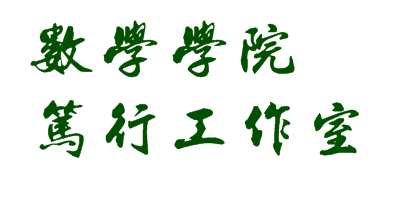
\includegraphics[height=0.7cm]{duxing_logo.png}}

\title{Neural Network}

\subtitle{A Selective Overview of Deep Learning}

\author{Tao Huang}

\date{}


\begin{document}
 
\frame{\titlepage}

\section{Feed-forward neural networks}

\begin{frame}{Model setup}
    Deep neural networks (DNNs) use composition of a series of simple nonlinear functions to model nonlinearity
    \begin{equation}
    \hh^{(L)} = \bg^{(L)} \circ  \bg^{(L-1)} \circ \ldots \circ \bg^{(1)} (\xx),
    \end{equation}
    \pause
    for $\ell = 1,\ldots,L$, define
    \begin{equation}\label{eq:fc}
        \hh^{(\ell)} = \bg^{(l)} \big(\bm{h}^{(l-1)}\big) \triangleq \bsigma \big(\bW^{(\ell)} \hh^{(\ell-1)} + \bb^{(\ell)}  \big),
    \end{equation}
    \pause
    The activation function $\bsigma(\cdot)$ is usually applied element-wise, and a popular choice is the ReLU (Rectified Linear Unit) function:
    \begin{equation}
        [\bsigma(\zz)]_j = \max\{ z_j, 0 \}.
    \end{equation} 
\end{frame}

\begin{frame}{Model setup}
    \begin{figure}
        \centering
        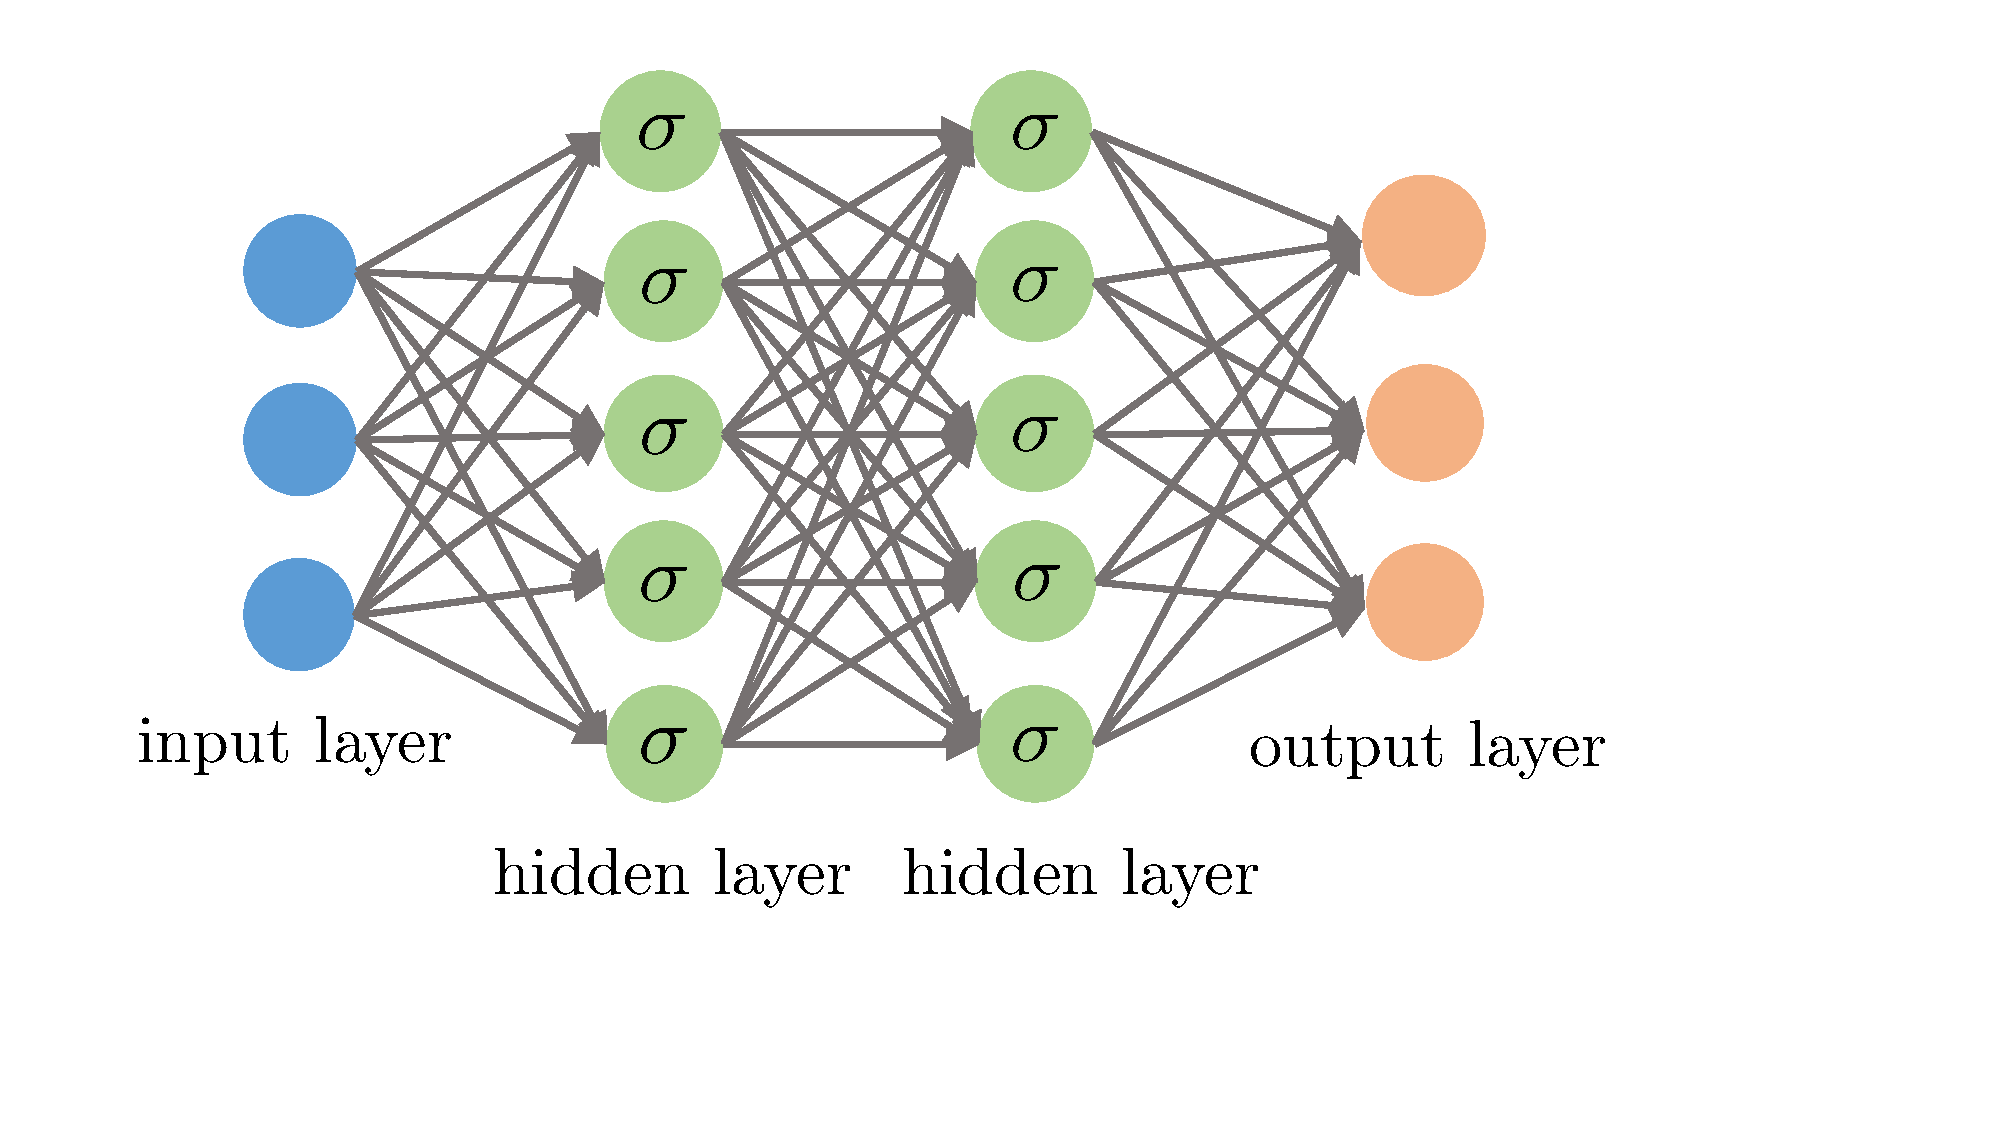
\includegraphics[scale=0.3]{MLP}\caption{A feed-forward neural network with an input layer, two hidden layers and an output layer. The input layer represents raw features $\{\bm{x}_{i}\}_{1\leq i\leq n}$. Both hidden layers compute an affine transform (a.k.s. indices) of the input and then apply an element-wise activation function $\bsigma(\cdot)$. Finally, the output returns a linear transform followed by the softmax activation (resp.~simply a linear transform) of the hidden layers for the classification (resp.~regression) problem. \label{fig:FFNN}}
    \end{figure}
\end{frame}

\begin{frame}{Model setup}
    The \textit{soft-max} function:
    \begin{equation}
        \begin{aligned}
            f_k(\xx; \btheta) \triangleq  \frac{\exp(z_k)}{\sum_k \exp(z_k)}, \, \forall\, k\in[K], \\ \where~ \zz = \bW^{(L+1)} \hh^{(L)} + \bb^{(L+1)} \in \mathbb{R}^{K}.
        \end{aligned}
    \end{equation}
    \pause
    Loss
    \begin{equation}\label{eq:crossentropy}
        \mathcal{L}(\ff(\xx; \btheta), y)=-\sum_{k=1}^K \bbone\{y = k\} \log p_k,
    \end{equation}
    ,where $\btheta \triangleq \{ \bW^{(\ell)}, \bb^{(\ell)}: 1\leq \ell \leq L+1\}$.
\end{frame}

\begin{frame}{Back-propagation\\ in computational graphs}
    The key to the above training procedure, namely SGD, is the calculation of the gradient $\nabla \ell_{\cB}(\btheta)$, where
    \begin{equation}\label{eq:loss-nn}
        \ell_{\cB}(\btheta) \triangleq |\cB|^{-1} \sum_{i \in \cB} \mathcal{L}(\ff(\xx_i ; \btheta), y_i).
    \end{equation}
    \pause
    \begin{equation}\label{eq:grad}
        \begin{aligned}
            \frac{\partial \ell_{\cB}}{\partial \hh^{(\ell-1)}} &=  \frac{\partial \hh^{(\ell)}}{\partial \hh^{(\ell-1)}} \cdot \frac{\partial \ell_{\cB}}{\partial \hh^{(\ell)}} \\
            & = (\bW^{(\ell)})^\top \mathsf{diag}\left( \bbone\{\bW^{(\ell)} \hh^{(\ell-1)} + \bb^{(\ell)}  \ge \bm{0}\}  \right) \frac{\partial \ell_{\cB}}{\partial \hh^{(\ell)}}
        \end{aligned}
    \end{equation}
\end{frame}

\begin{frame}{Back-propagation\\ in computational graphs}
    \begin{equation}\label{eq:Wupdate}
        \bW^{(\ell)} \leftarrow \bW^{(\ell)} - \eta \frac{\partial \ell_{\cB}}{\partial \bW^{(\ell)}}, \, \where \, \frac{\partial \ell_{\cB}}{\partial W_{jm}^{(\ell)}} = \frac{\partial \ell_{\cB}}{\partial h_j^{(\ell)}} \cdot \sigma' \cdot h_m^{(\ell-1)},
    \end{equation}
    \pause
    MLP with a single hidden layer and an $\ell_2$ regularization:
    \begin{equation}\label{eq:regloss}
    \ell_{\cB}^\lambda (\btheta) = \ell_{\cB}(\btheta) + r_\lambda(\btheta) = \ell_{\cB}(\btheta) + \lambda \Big( \sum_{j,j'} \big(W_{j,j'}^{(1)}\big)^2 + \sum_{j,j'} \big(W_{j,j'}^{(2)}\big)^2 \Big),
    \end{equation}
\end{frame}

\begin{frame}{Back-propagation\\ in computational graphs}
    \begin{figure}[t]
        \centering
        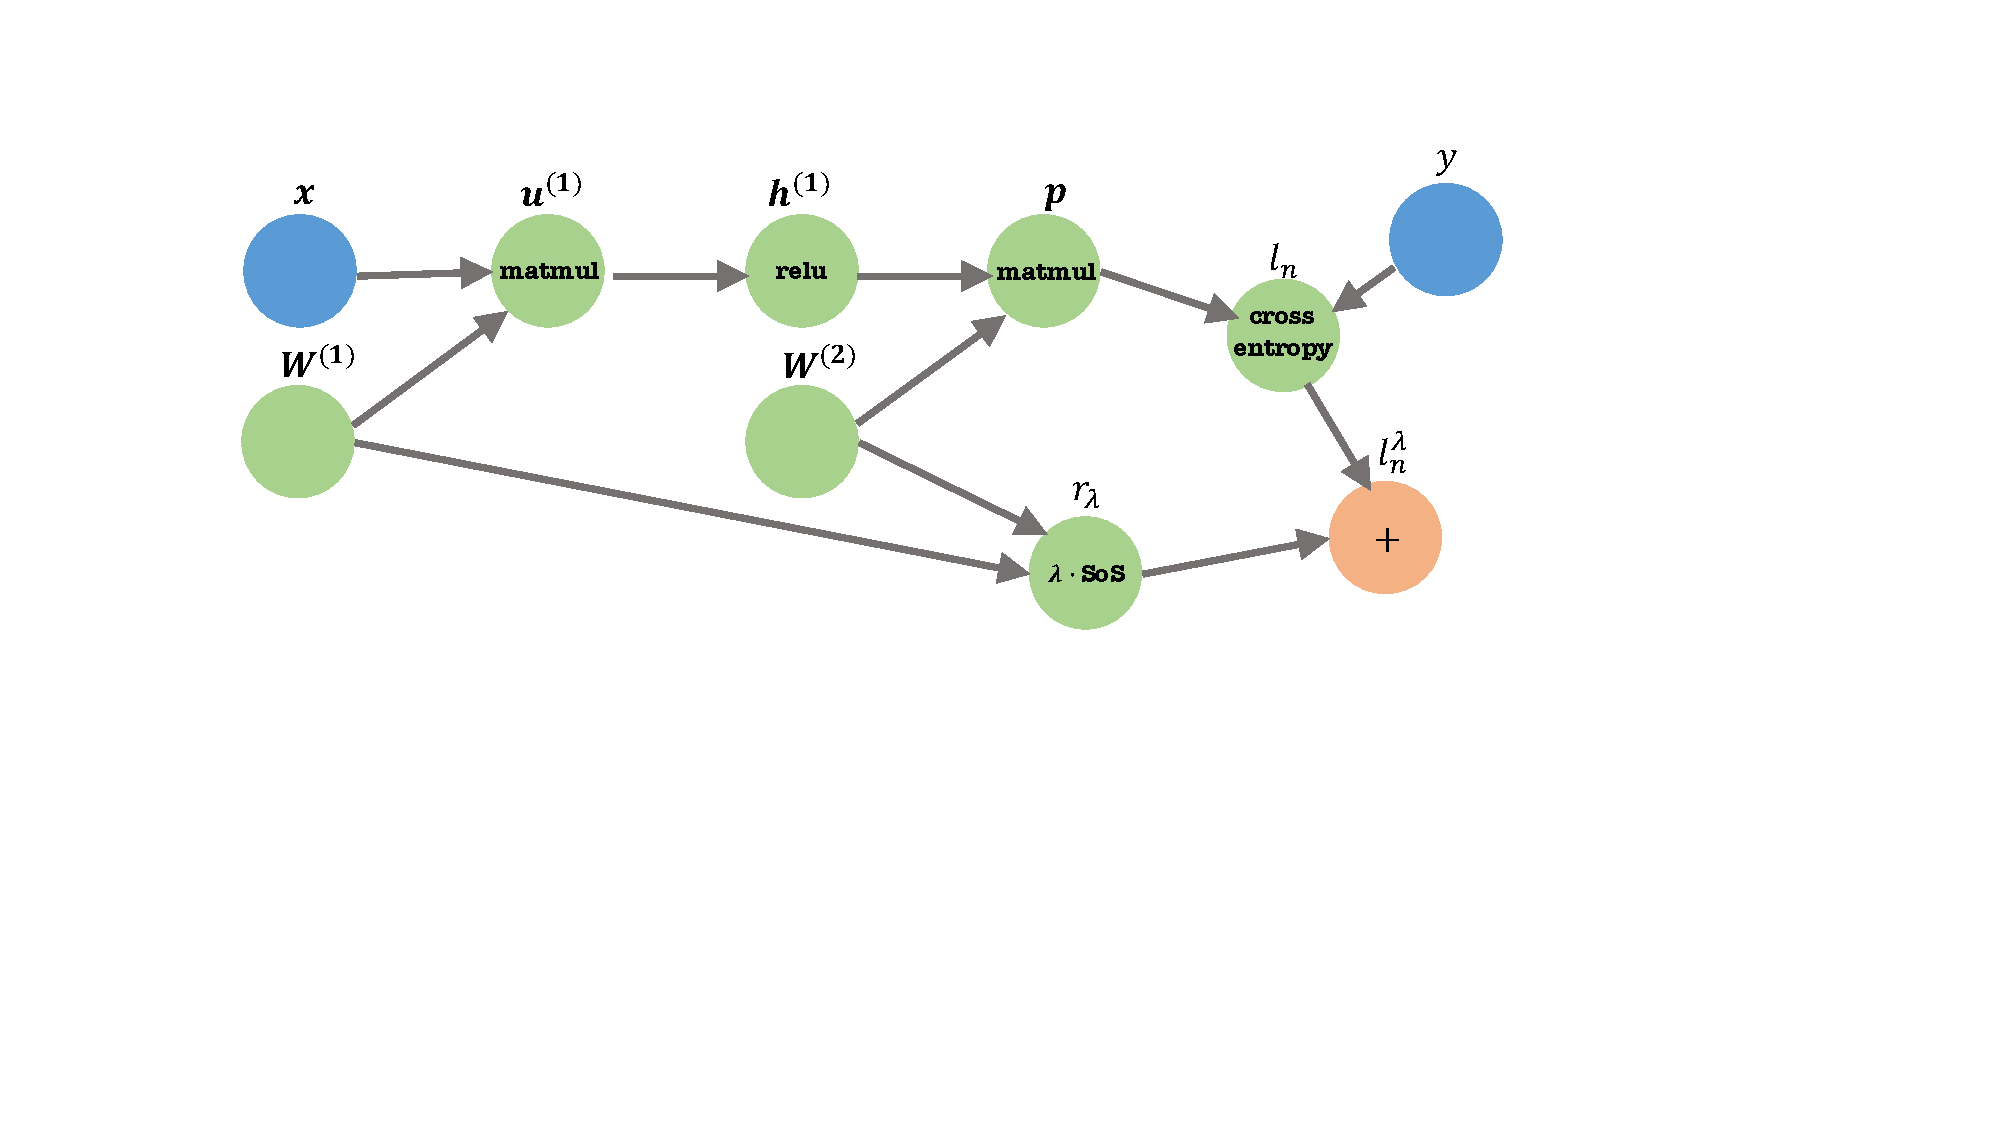
\includegraphics[width=0.75\textwidth]{compuGraph2}\caption{The computational graph illustrates the loss \eqref{eq:regloss}. For simplicity, we omit the bias terms. Symbols inside nodes represent functions, and symbols outside nodes represent function outputs (vectors/scalars). {\normalfont \texttt{matmul}} is matrix multiplication, {\normalfont \texttt{relu}} is the ReLU activation, {\normalfont \texttt{cross entropy}} is the cross entropy loss, and {\normalfont \texttt{SoS}} is the sum of squares.} \label{fig:comgraph}
    \end{figure}
\end{frame}


\begin{frame}{Numerical experiments}
    
\end{frame}

\section{Convolutional neural networks}


\begin{frame}{Convolutional layer (CONV)}
    \begin{equation}\label{eq:conv}
        O^{k}_{ij}= \big\langle \left[\bm{X}\right]_{ij}, \bm{F}_{k} \big\rangle = \sum_{i'=1}^w \sum_{j'=1}^w \sum_{l=1}^{d_3} [\bm{X}]_{i+i'-1, j+j'-1, l} [\bm{F}_{k}]_{i',j',l}.
    \end{equation}
    \pause
    \begin{equation}\label{eq:relu}
    \tilde{X}_{ijk} = \sigma(O_{ijk}), \, \forall\, i \in [d_1-w+1], j \in [d_2-w+1], k \in [\tilde d_3].
    \end{equation}
\end{frame}

\begin{frame}{Convolutional layer}
    \begin{figure}
    \centering
    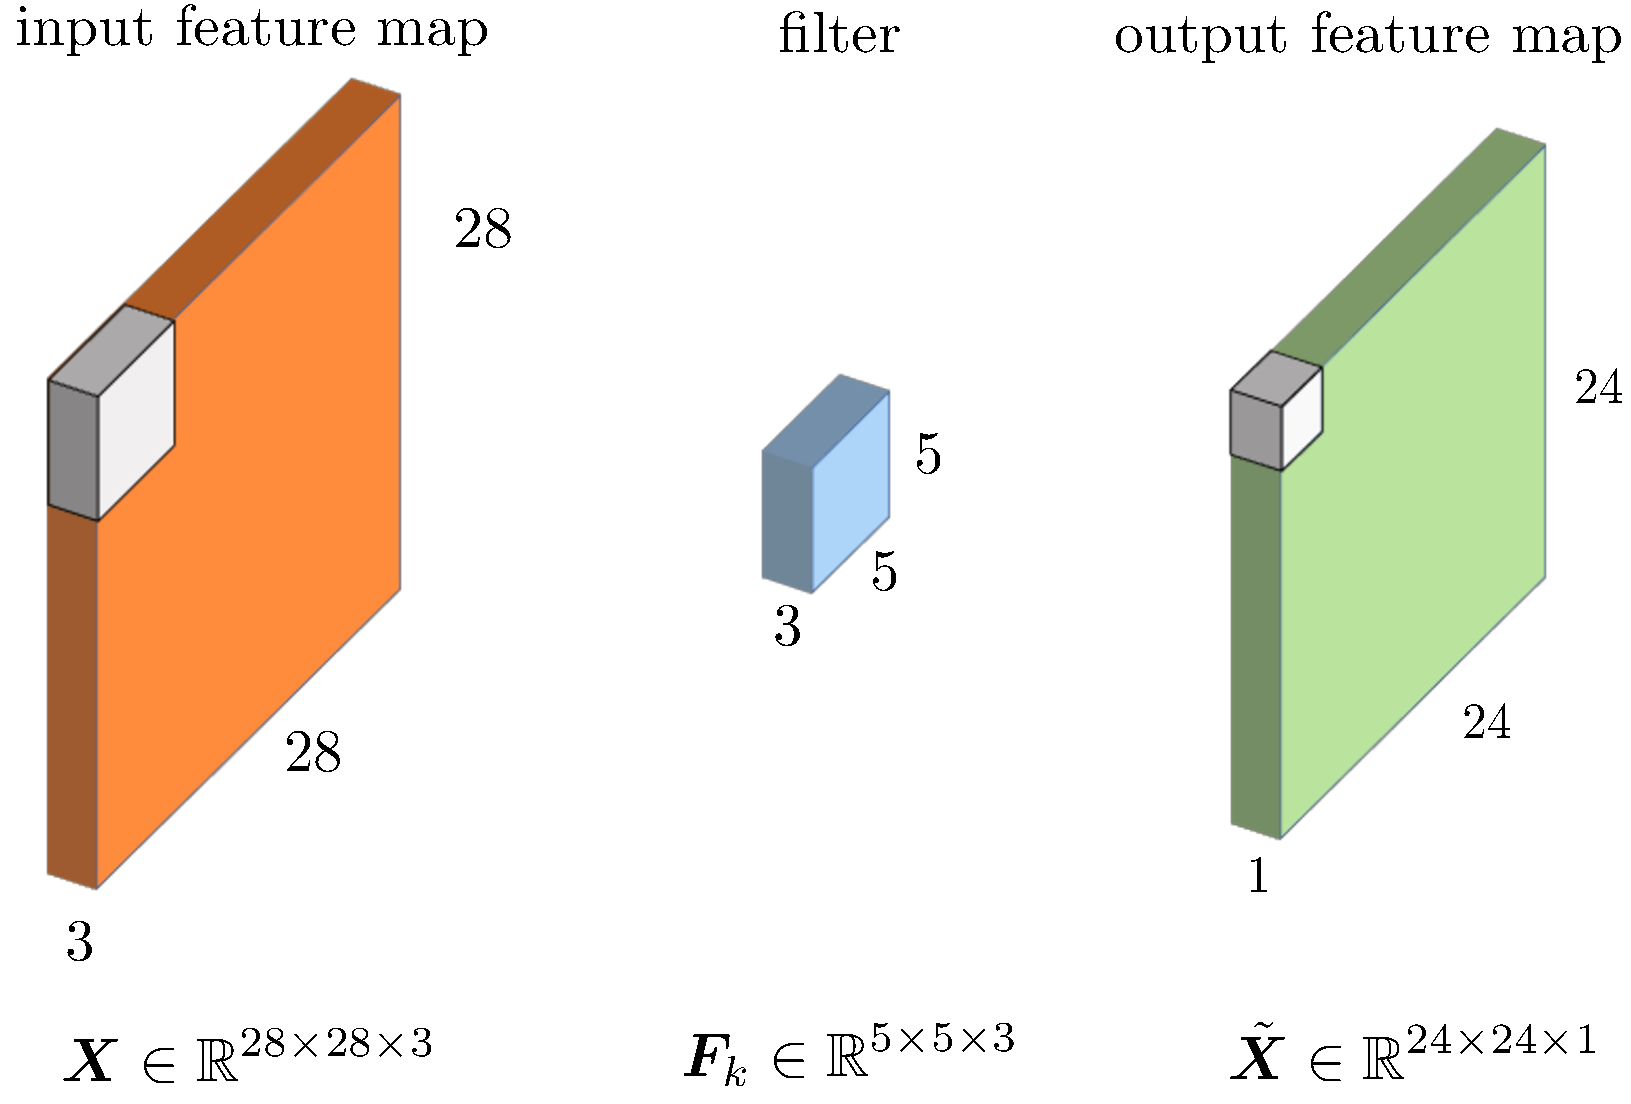
\includegraphics[height=0.4\textwidth]{convolution_3D}

    \caption{$\bm{X}\in \mathbb{R}^{28\times 28 \times 3}$ represents the input feature consisting of $28 \times 28$ spatial coordinates in a total number of 3  channels / feature maps. $\bm{F}_{k}\in\mathbb{R}^{5\times 5 \times 3}$ denotes the $k$-th filter with size $5\times 5$. The third dimension $3$ of the filter automatically matches the number $3$  of channels in the previous input. Every 3D patch of $\bm{X}$ gets convolved with the filter $\bm{F}_{k}$ and this as a whole results in a single output feature map $\tilde{X}_{:,:,k}$ with size $24\times 24\times 1$. Stacking the outputs of all the filters $\{\bm{F}_{k}\}_{1\leq k\leq K}$ will lead to the output feature with size $24\times 24\times K$. \label{fig:Convolution-operation}}

    \end{figure}
\end{frame}


\begin{frame}{Pooling layer (POOL)}
    \begin{figure}
    \centering
    
    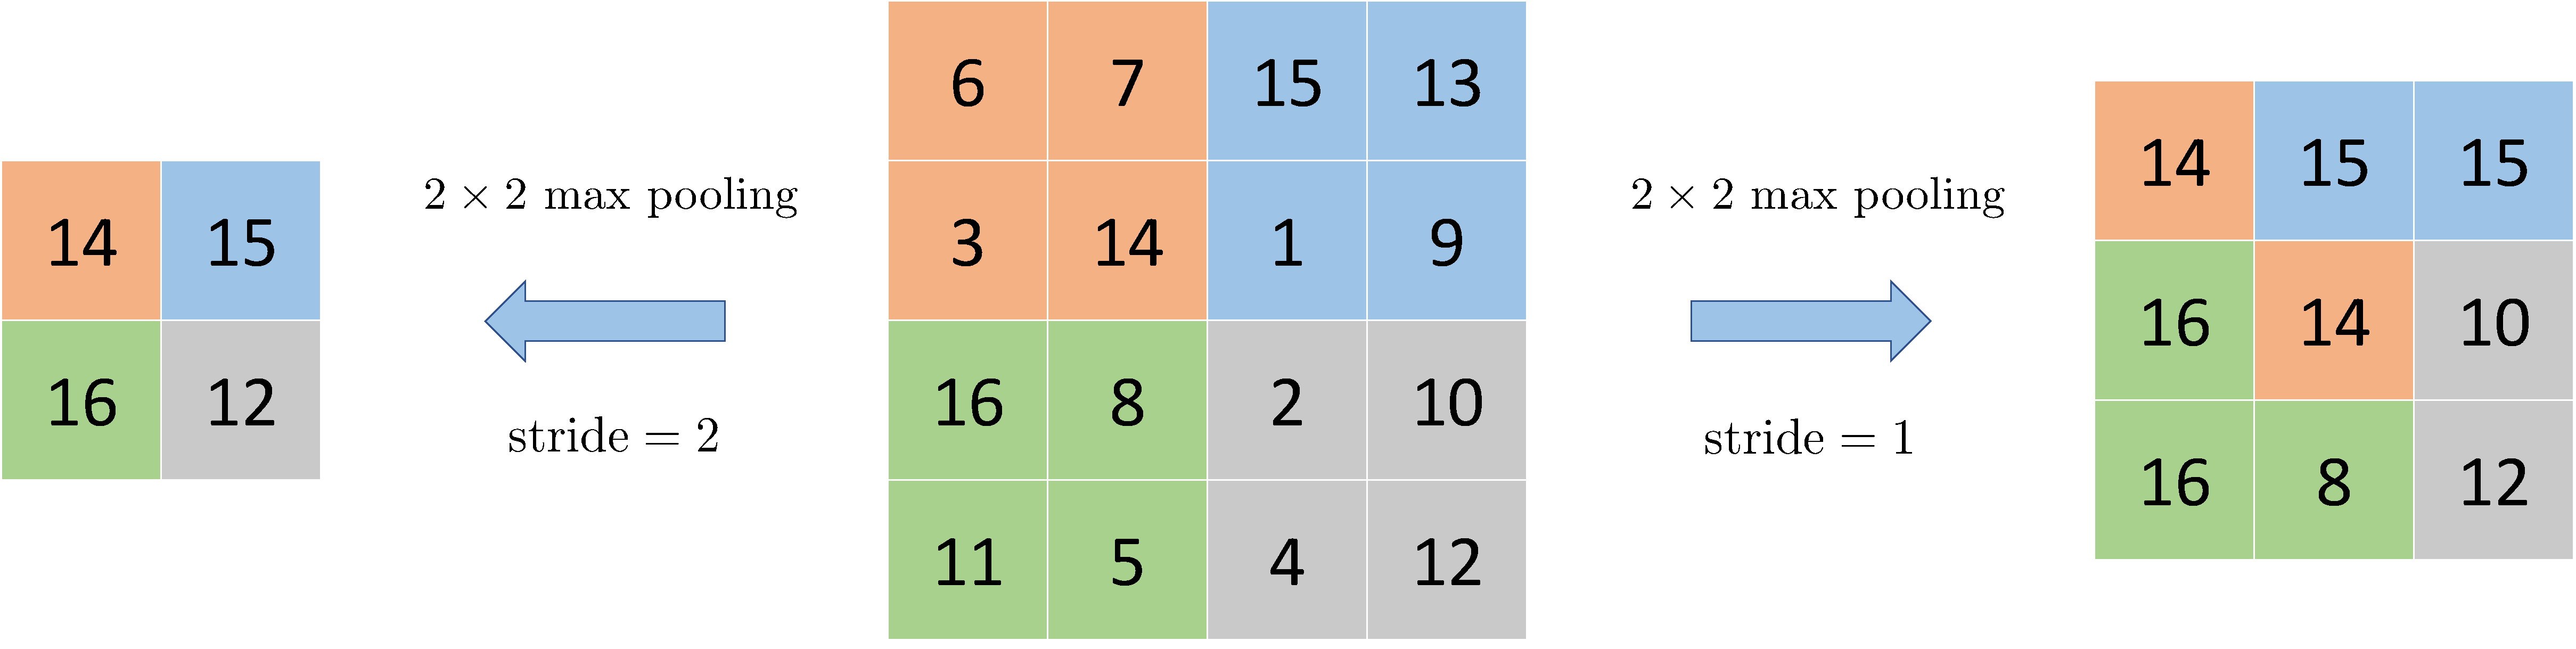
\includegraphics[width=0.95 \linewidth]{pooling}\caption{A $2\times 2$ max pooling layer extracts the maximum of 2 by 2 neighboring pixels$\,$/$\,$features across the spatial dimension. }\label{fig:pooling}
    \end{figure}
\end{frame}

\begin{frame}{LeNet}
    \begin{figure}
    \centering
    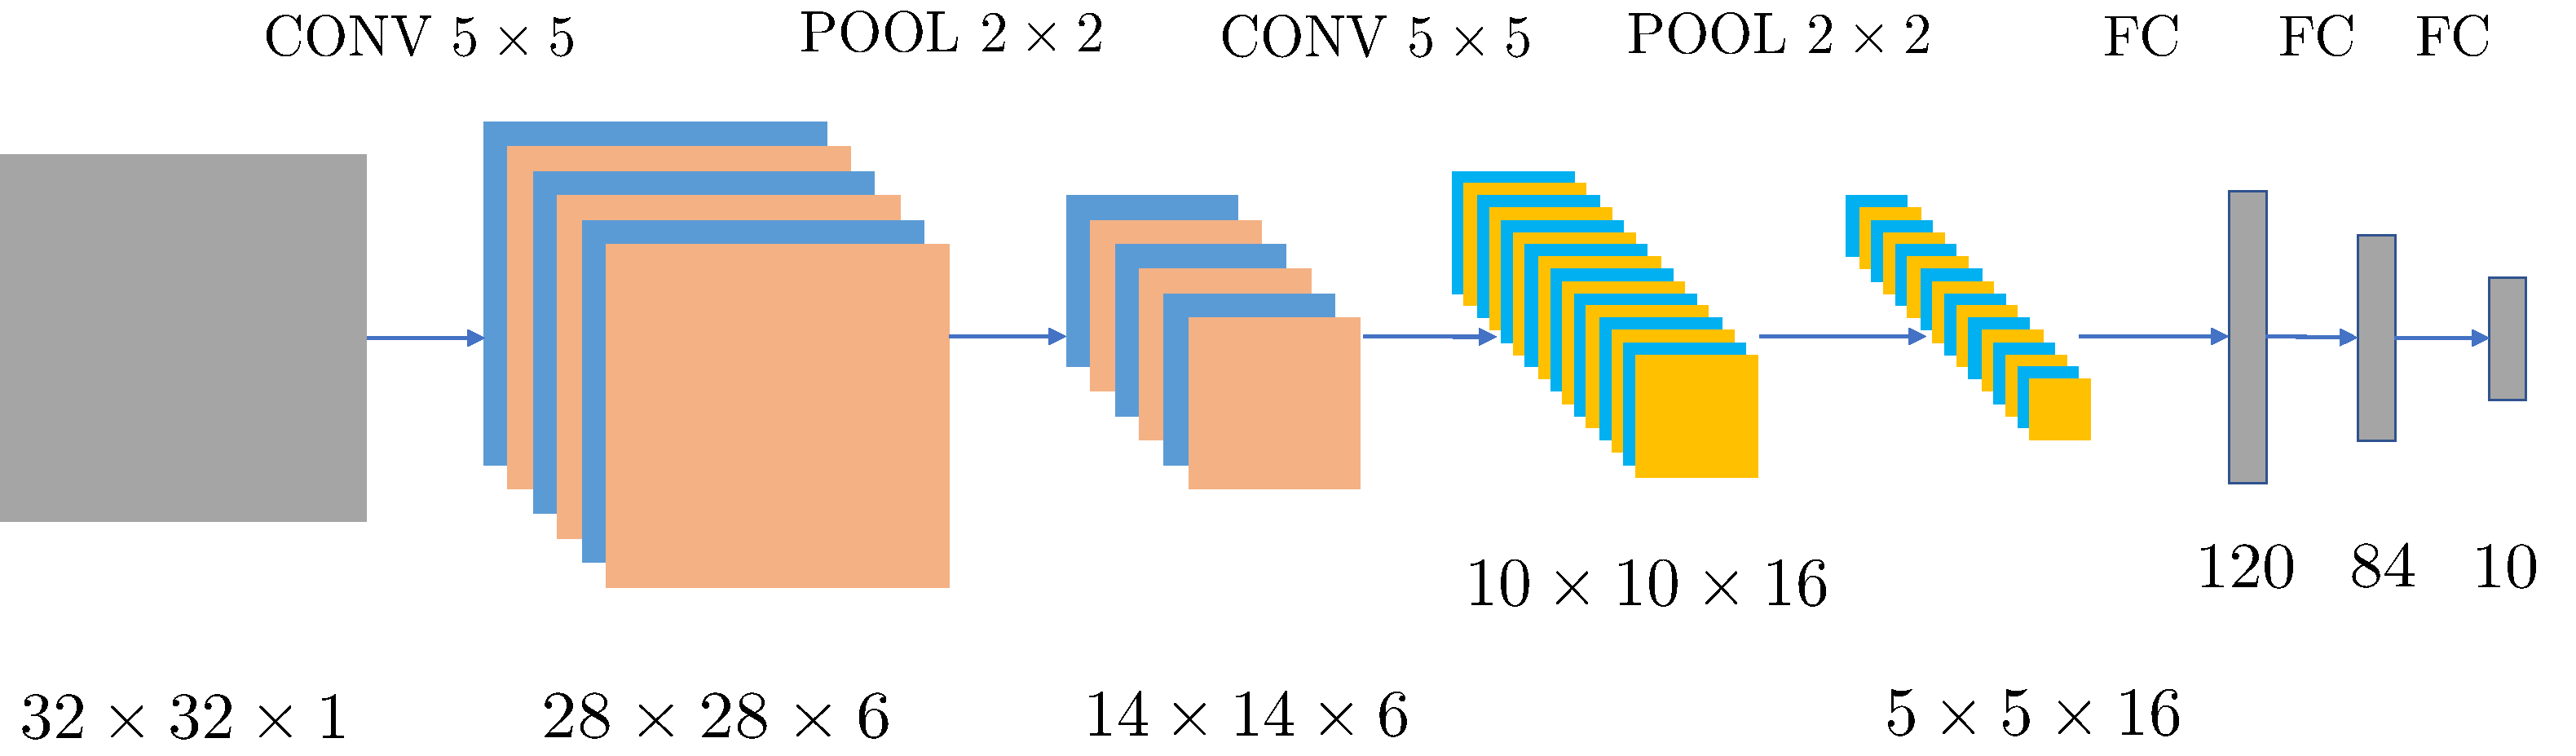
\includegraphics[width=0.9 \textwidth]{LeNet}\caption{LeNet is composed of an input layer, two convolutional layers, two pooling layers and three fully-connected layers. Both convolutions are valid and use filters with size $5 \times 5$. In addition, the two pooling layers use $2 \times 2$ average pooling. \label{fig:CNN}}
    \end{figure}
    
\end{frame}


\begin{frame}{Numerical experiments}
    
\end{frame}

\section{Recurrent neural networks}

\begin{frame}{Vanilla RNNs}
    \begin{figure}
    \centering
    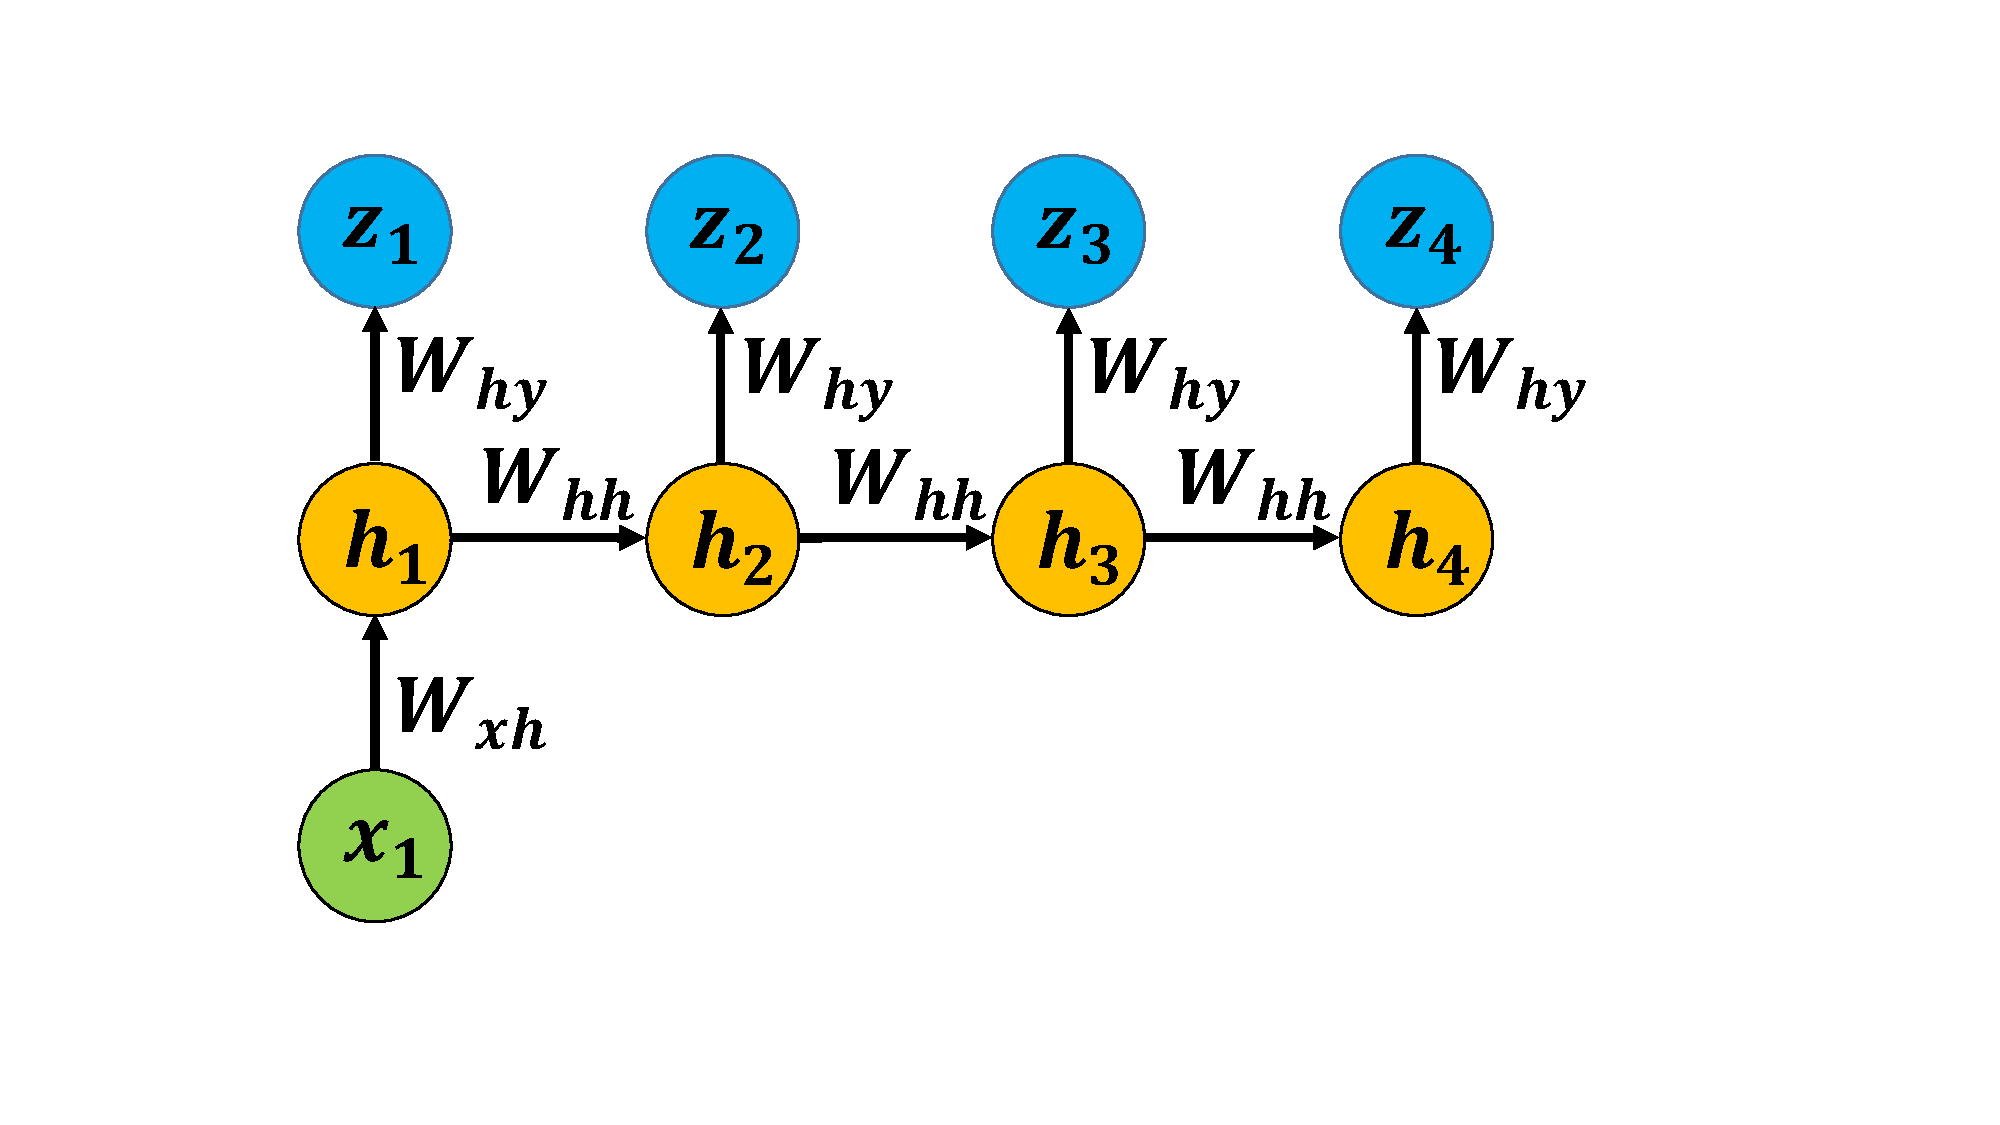
\includegraphics[width=0.8 \textwidth]{RNN1-1}
    \caption{Vanilla RNNs with different inputs/outputs settings. (a) has one input but multiple outputs; }
    \end{figure}
\end{frame}

\begin{frame}{Vanilla RNNs}
    \begin{figure}
    \centering
    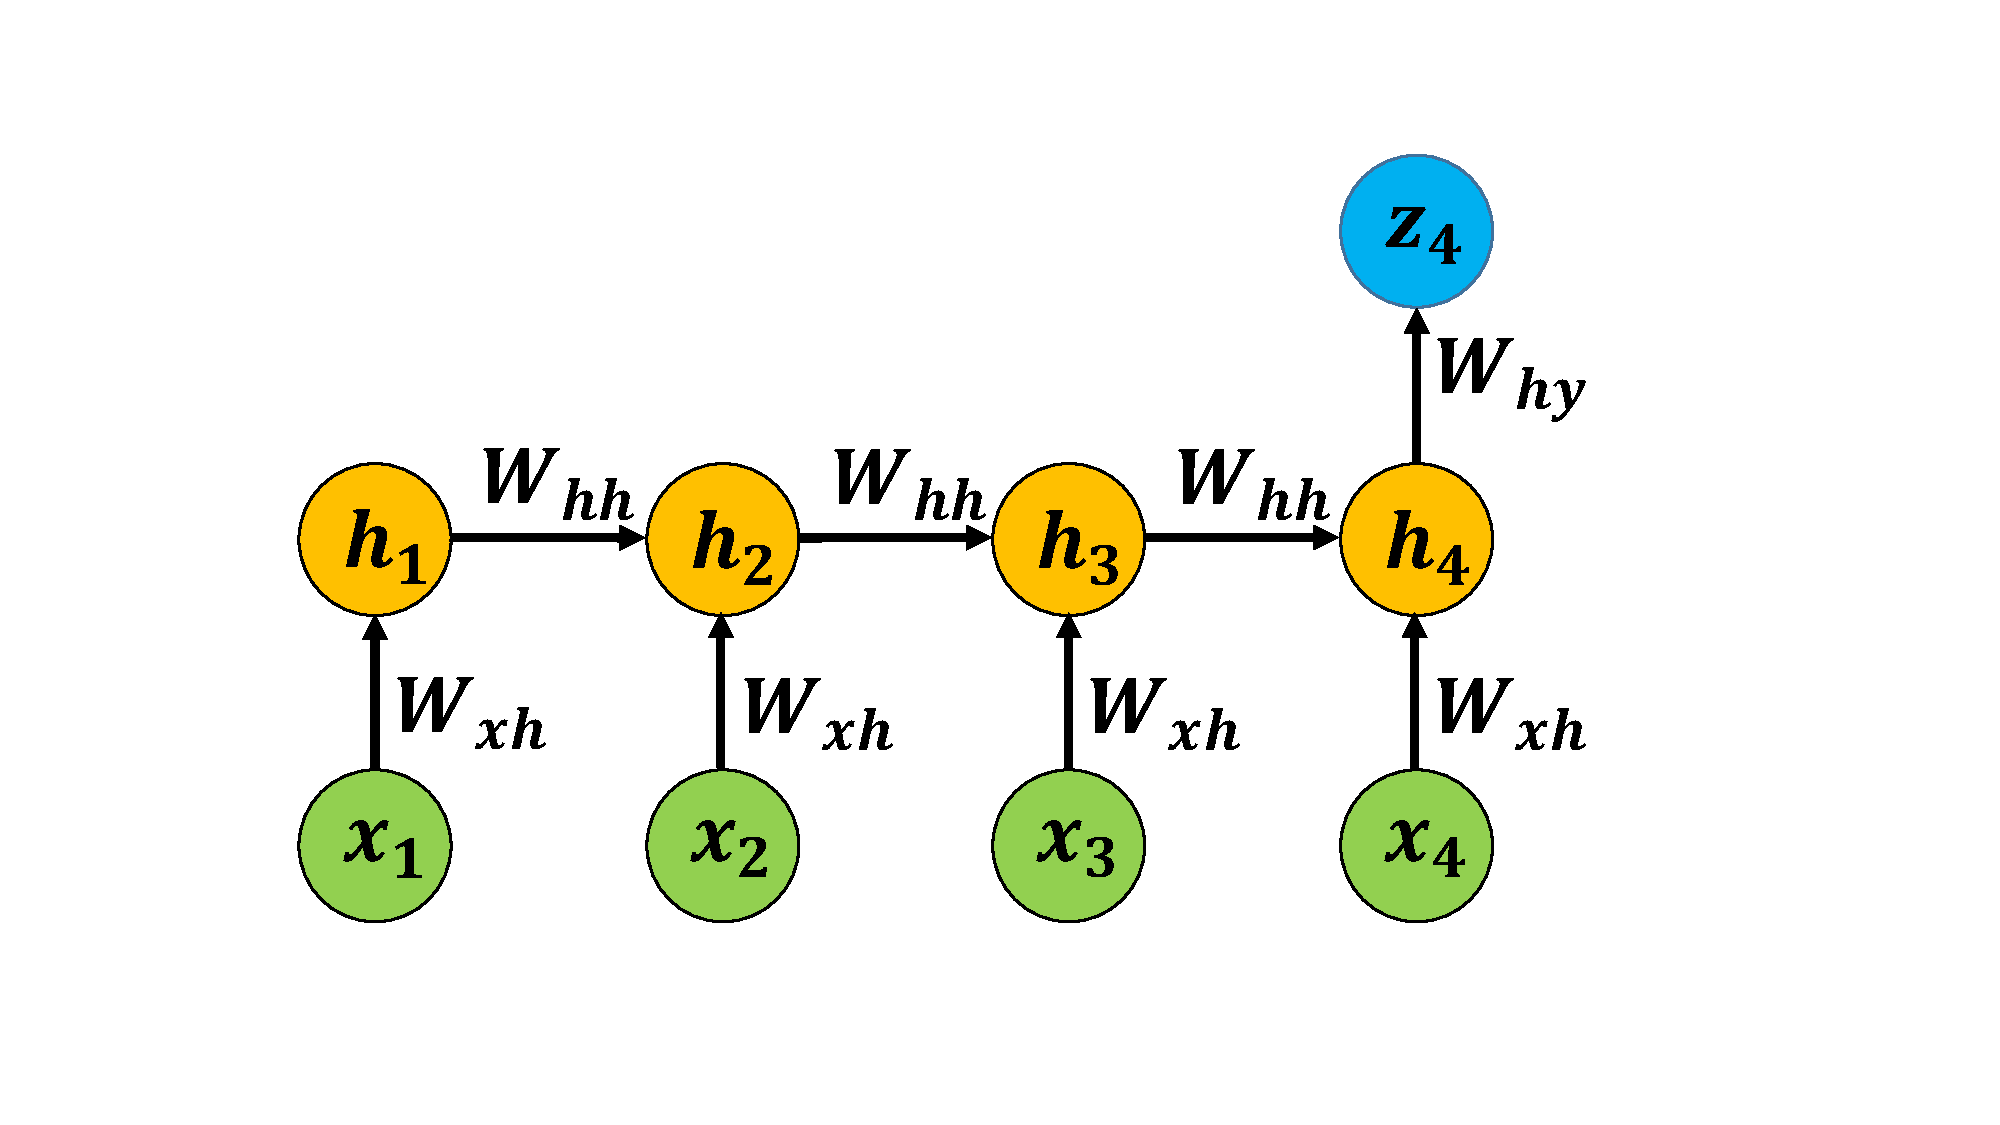
\includegraphics[width=0.8 \textwidth]{RNN1-2}
    \caption{Vanilla RNNs with different inputs/outputs settings.(b) has multiple inputs but one output; }
    \end{figure}
\end{frame}

\begin{frame}{Vanilla RNNs}
    \begin{figure}
    \centering
    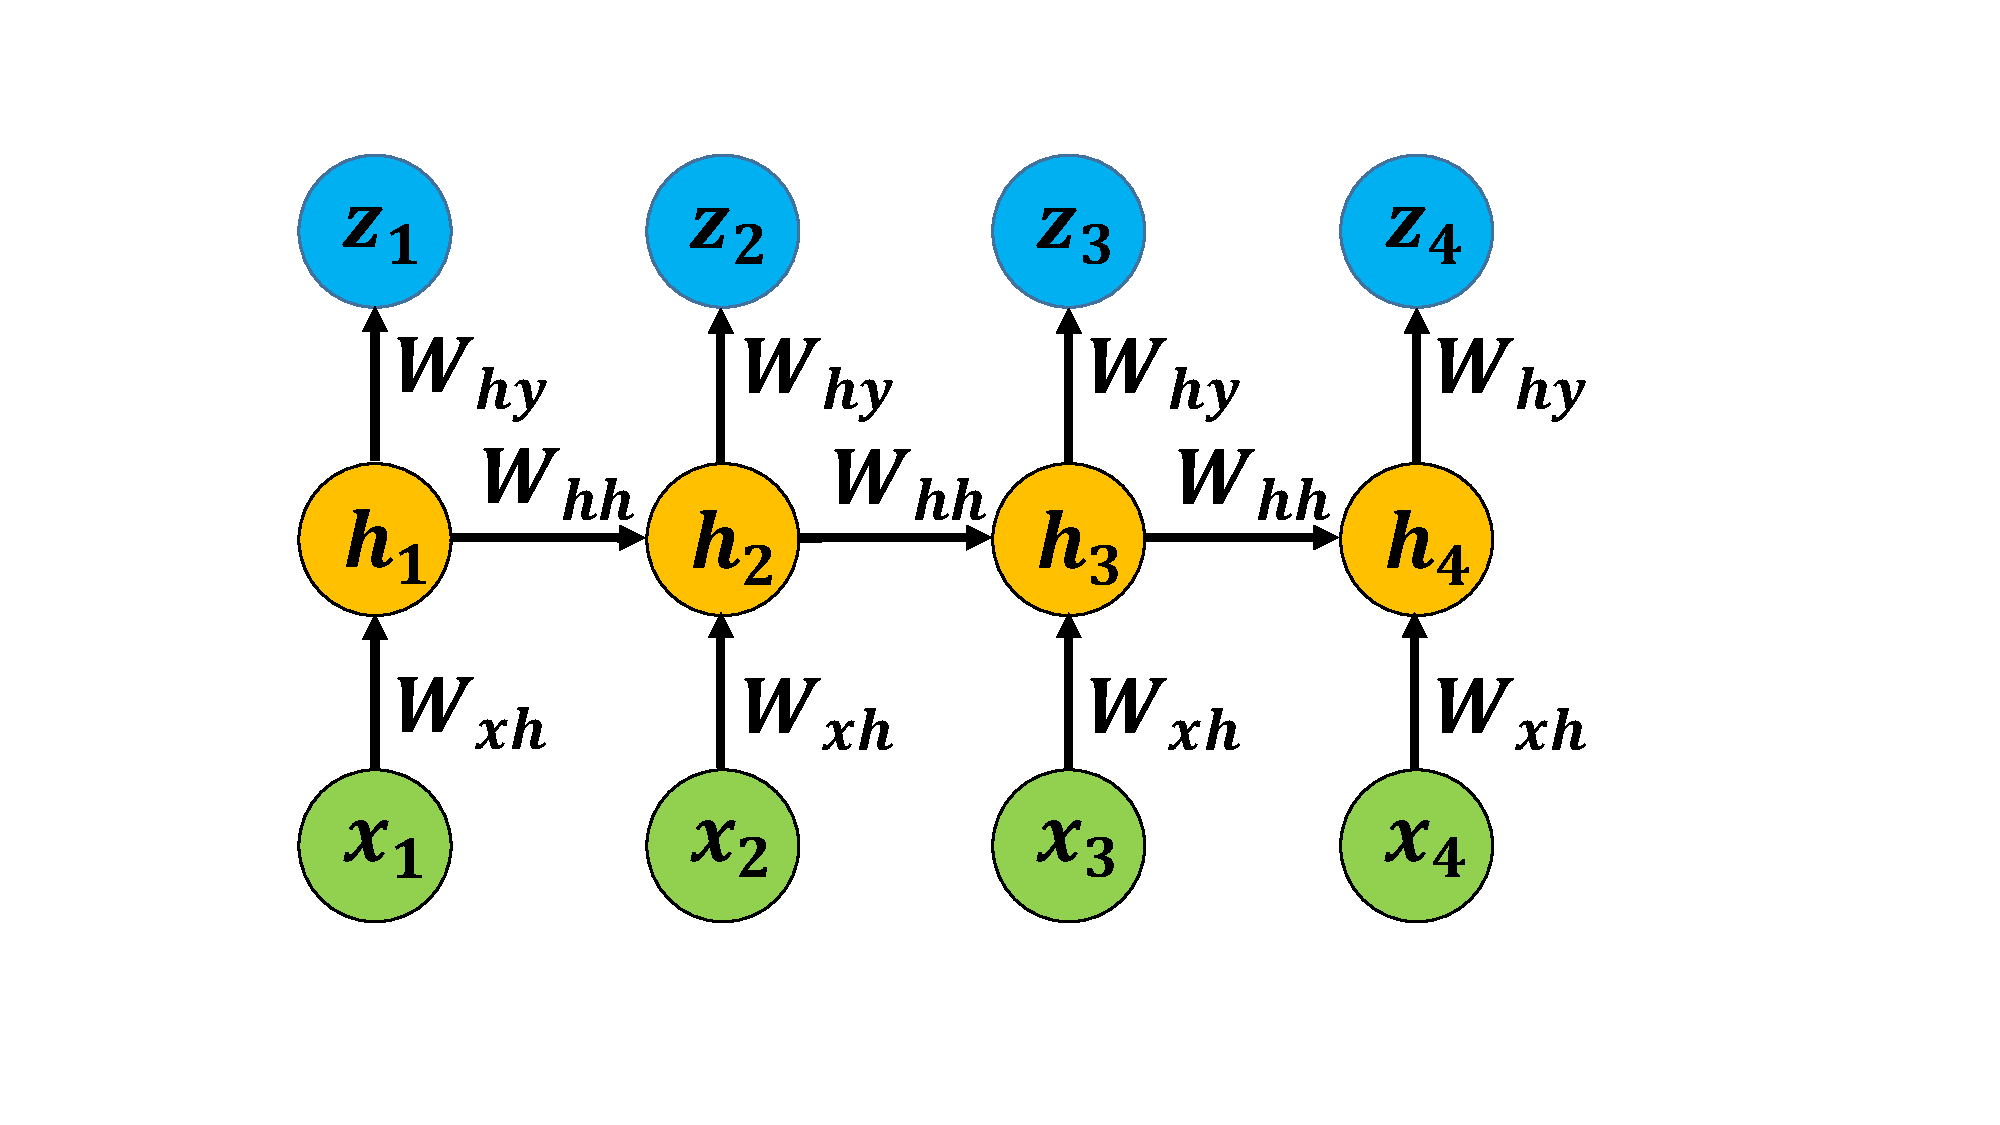
\includegraphics[width=0.8 \textwidth]{RNN1-3}
    \caption{Vanilla RNNs with different inputs/outputs settings. (c) has multiple inputs and outputs. Note that the parameters are shared across time steps.}
    \end{figure}
\end{frame}

\begin{frame}{Vanilla RNNs}
    
    \begin{equation}
        \hh_t = \ff_{\btheta}(\hh_{t-1}, \xx_t).
    \end{equation}
    \pause
    \begin{align}
        \hh_t  &= \btanh\left( \bW_{hh} \hh_{t-1}+ \bW_{xh} \xx_t + \bb_\hh \right), \\
        \tanh(a) &= \frac{e^{2a} - 1}{e^{2a} + 1}, \\
        \zz_t &= \bsigma \left(\bW_{hy} \hh_t + \bb_\zz \right),
    \end{align}
    \pause
    \begin{equation}
        \begin{aligned}
            \ell_{\cT}(\btheta) &= \sum_{t \in \cT} \cL(y_t, \zz_t) \\
             &= - \sum_{t \in \cT} \sum_{k=1}^K \bbone\{y_t = k\} \log \left( \frac{\exp([\zz_t]_k)}{\sum_k \exp([\zz_t]_k)} \right),
        \end{aligned}
    \end{equation}
\end{frame}

\begin{frame}
    \frametitle{LSTM}
    \begin{align}
        \left( \begin{array}{c} \ii_t \\ \ff_t \\ \oo_t \\ \bgg_t \end{array} \right) &= \left( \begin{array}{c} \bsigma \\ \bsigma \\ \bsigma \\ \btanh \end{array} \right) \bW \left( \begin{array}{c} \hh_{t-1} \\ \xx_t \\ 1 \end{array} \right), \\
        \cc_t &= \ff_t \odot \cc_{t-1} + \ii_t \odot \bgg_t, \\
        \hh_t &= \oo_t \odot \btanh(\cc_t),
    \end{align}
\end{frame}

\begin{frame}
    \frametitle{Multilayer RNNs}
    
    \begin{equation}
        \hh_t^{\ell} =  \btanh \left[\bW^\ell \left( \begin{array}{c} \hh_t^{\ell-1} \\ \hh_{t-1}^\ell \\ 1 \end{array} \right) \right], \quad \text{for all}\, \ell \in [L], \qquad \hh_t^{0} \triangleq \xx_t.
    \end{equation}

\end{frame}

\begin{frame}
    \frametitle{Multilayer RNNs}
    \begin{figure}
        \centering
        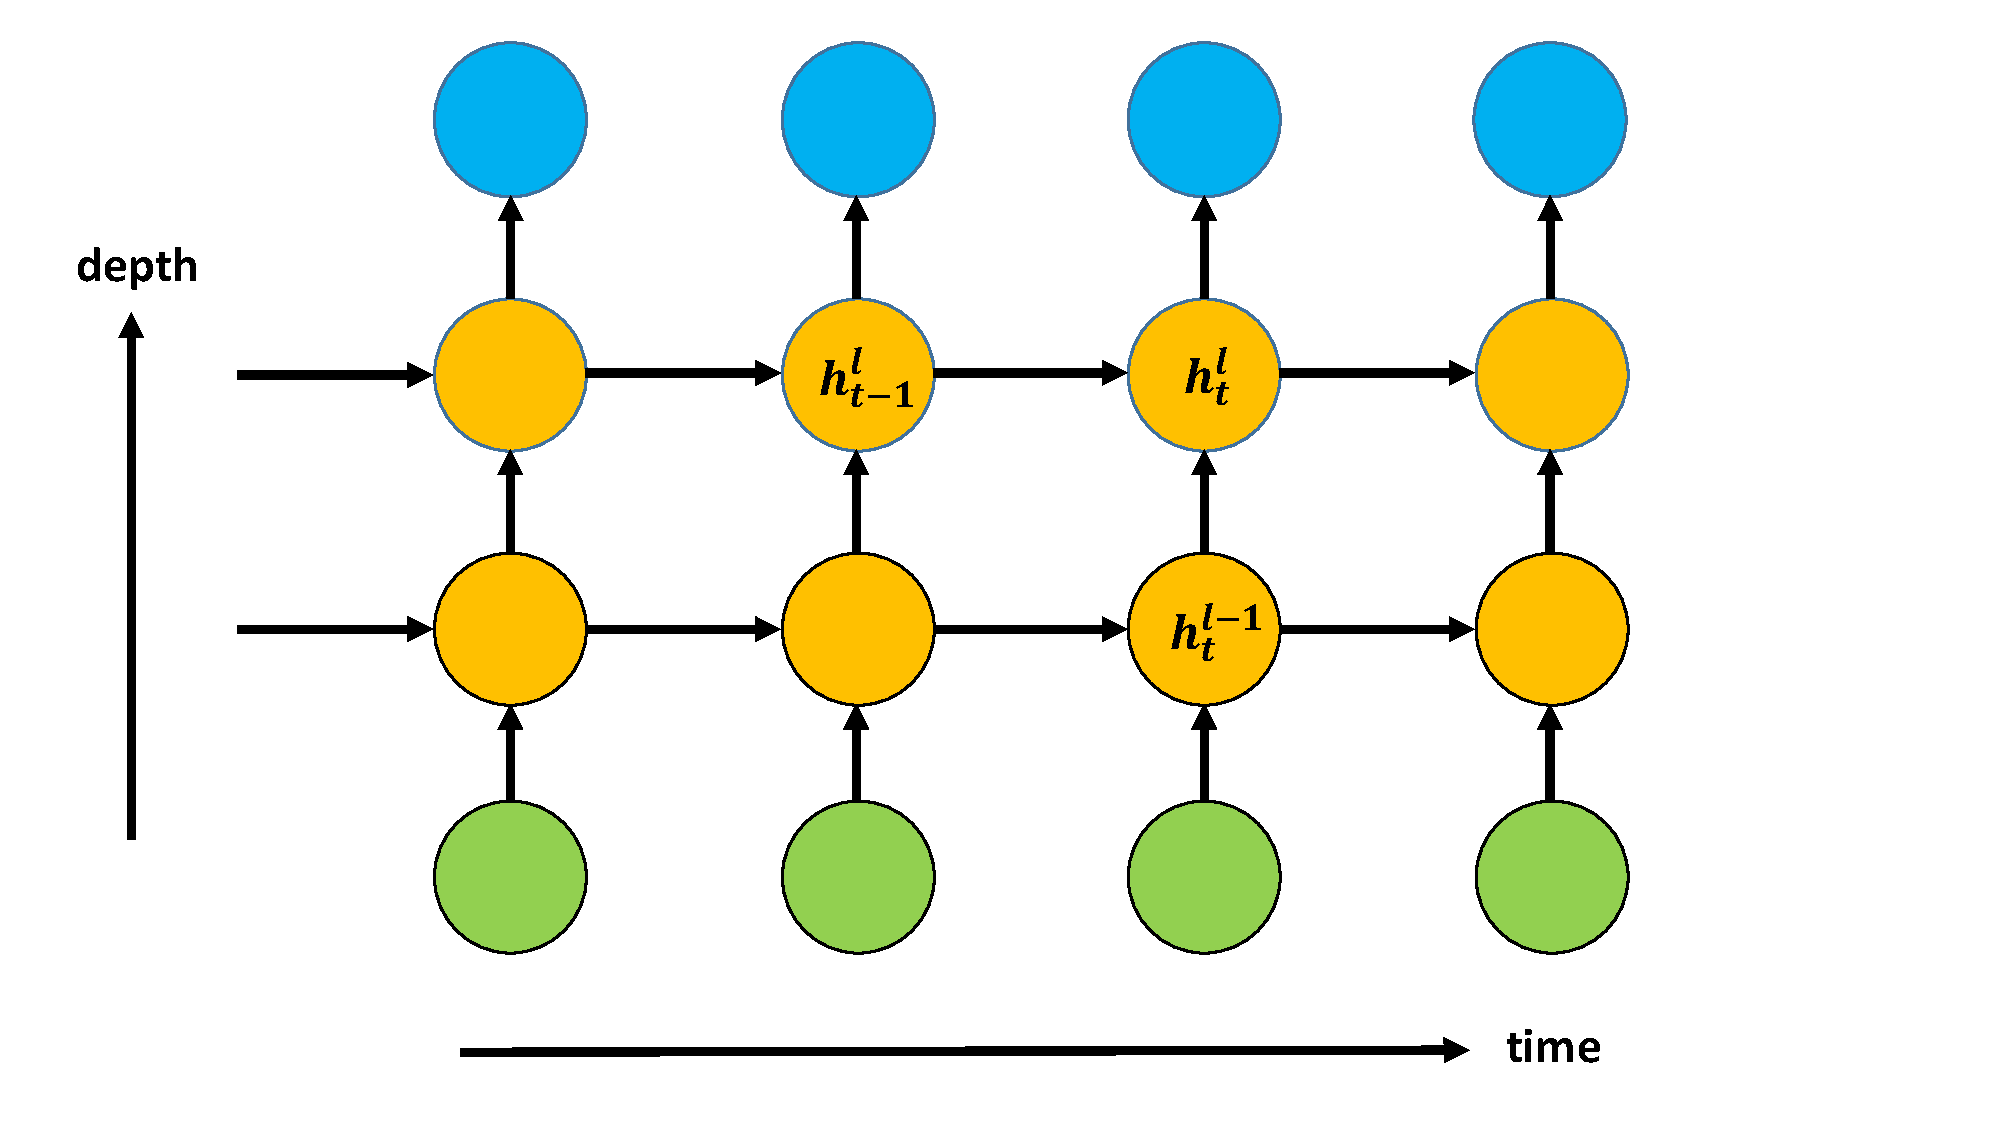
\includegraphics[width = 0.7\textwidth]{RNN2}
        \caption{A vanilla RNN with two hidden layers. Higher-level hidden states $\hh_t^{\ell}$ are determined by the old states $\hh_{t-1}^\ell$ and lower-level hidden states $\hh_t^{\ell-1}$. Multilayer RNNs generalize both feed-forward neural nets and one-hidden-layer RNNs.}\label{fig:RNN2}
    \end{figure}

\end{frame}


\section{Modules}

\begin{frame}
    \frametitle{Skip connections}
    \begin{figure}[htb!]
        \centering
        \begin{tabular}{cc}
        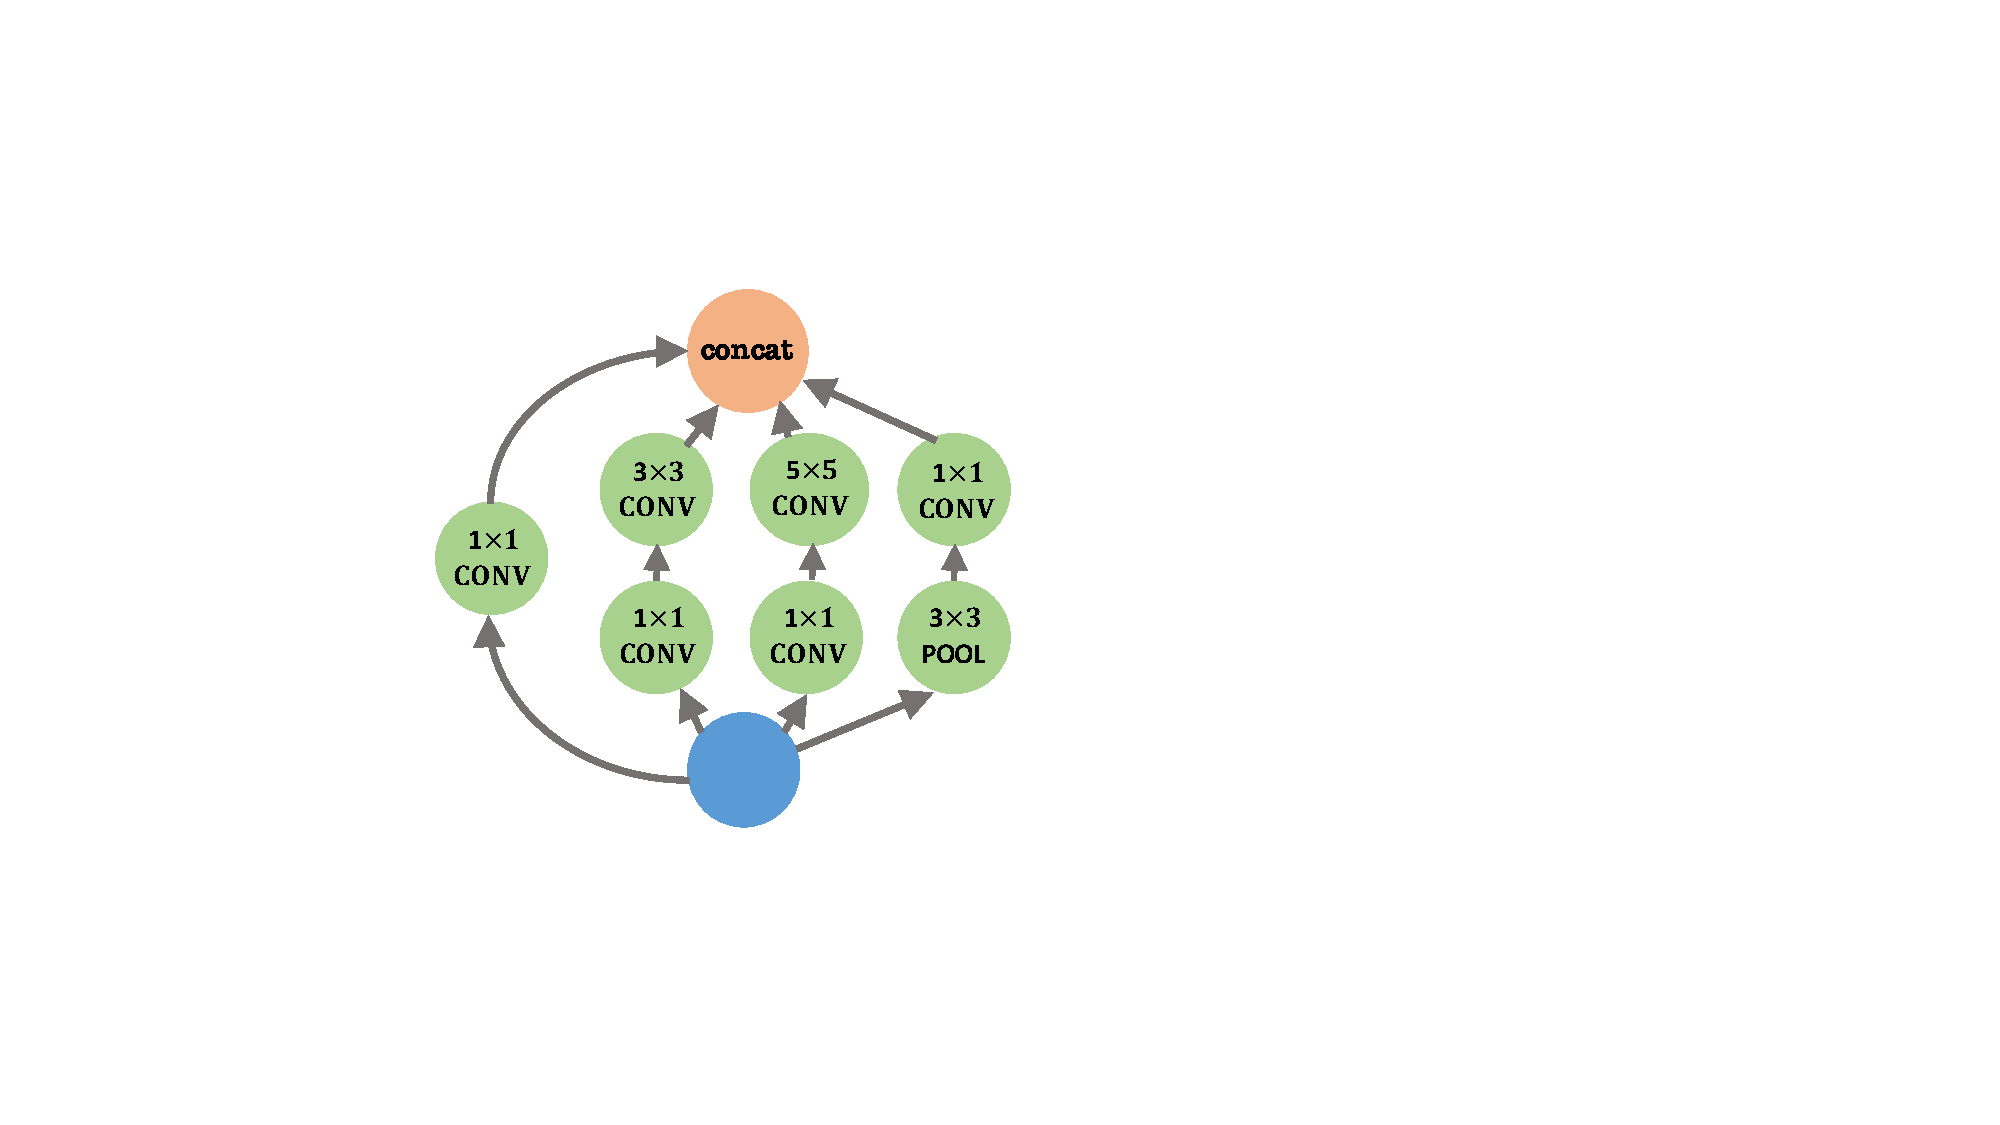
\includegraphics[scale = 0.5]{inception} & 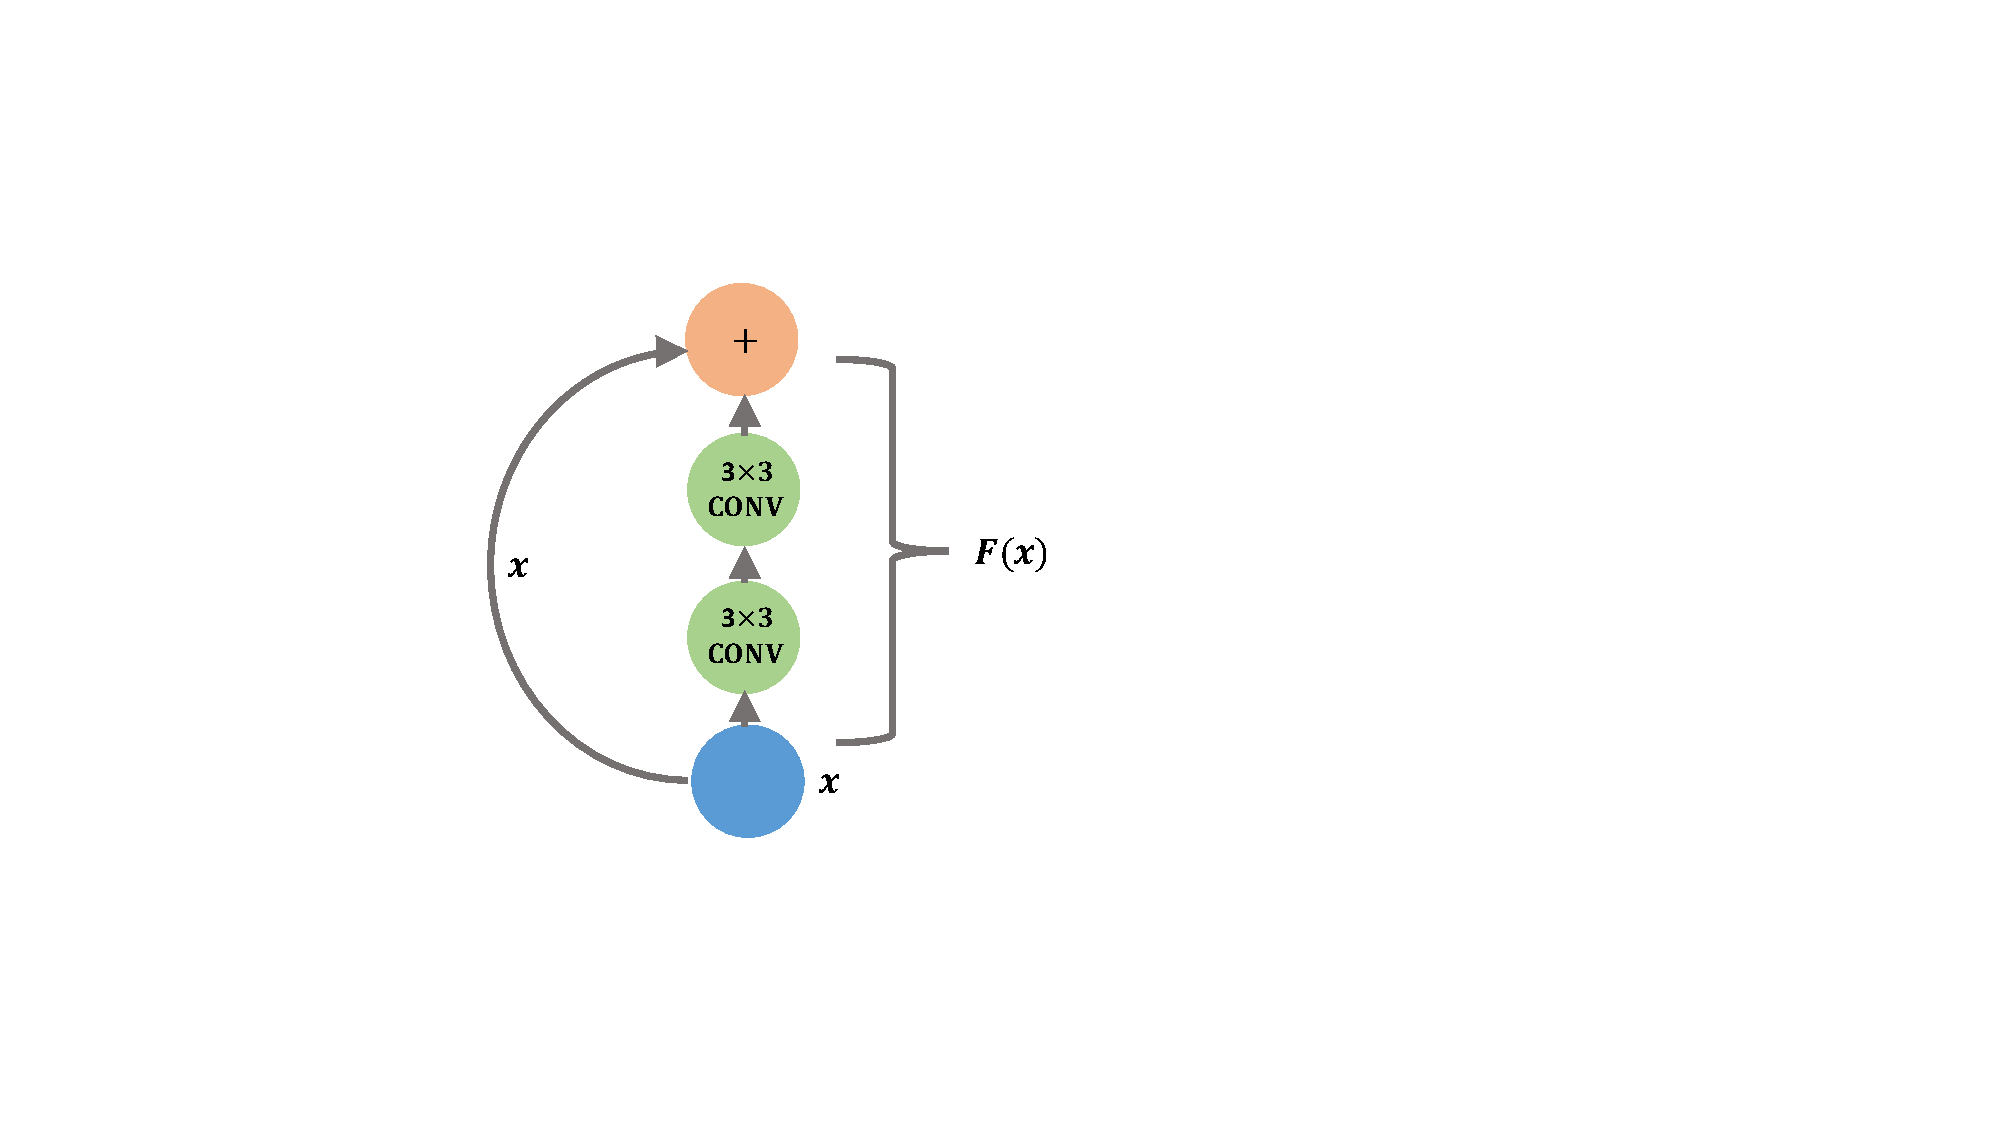
\includegraphics[scale = 0.5]{resnet2} \tabularnewline
        (a) ``Inception'' module & (b) Skip connections
        \end{tabular}
        \caption{(a) The ``Inception'' module from GoogleNet. \texttt{Concat} means combining all features maps into a tensor. (b) Skip connections are added every two layers in ResNets. }\label{fig:skip}
    \end{figure}

\end{frame}

\begin{frame}
    \frametitle{Skip connections}

    \begin{equation}\label{eq:mapsto}
        \xx \longmapsto \bsigma(\xx + \bF(\xx)) = \bsigma(\xx + \bW' \bsigma(\bW \xx + \bb) + \bb'),
    \end{equation}

\end{frame}

\section{Autoencoders}

\begin{frame}
    \frametitle{Autoencoders}

    \begin{align}
        \ff\left(\bm{x}\right)& =\bm{W}_f\bm{x}\triangleq \hh \\
        \bgg\left(\bm{h}\right)& =\bm{W}_g\bm{h}, \\
        \bm{W}_f\in\mathbb{R}^{k\times d} & \text{and}  \bm{W}_g\in\mathbb{R}^{d\times k}.
    \end{align}
    \pause
    
    \begin{equation}
        \min _{\ff,\bgg} \quad\frac{1}{n}\sum_{i=1}^{n}\mathcal{L}\left(\bm{x}_{i},\bgg\left(\bm{h}_{i}\right)\right) \, \text{with} \, \bm{h}_{i}=\ff\left(\bm{x}_{i}\right), \, \forall i \in [n].  \label{eq:AE}
    \end{equation}
\end{frame}

\begin{frame}
    \frametitle{Autoencoders}

    
    \begin{figure}
        \centering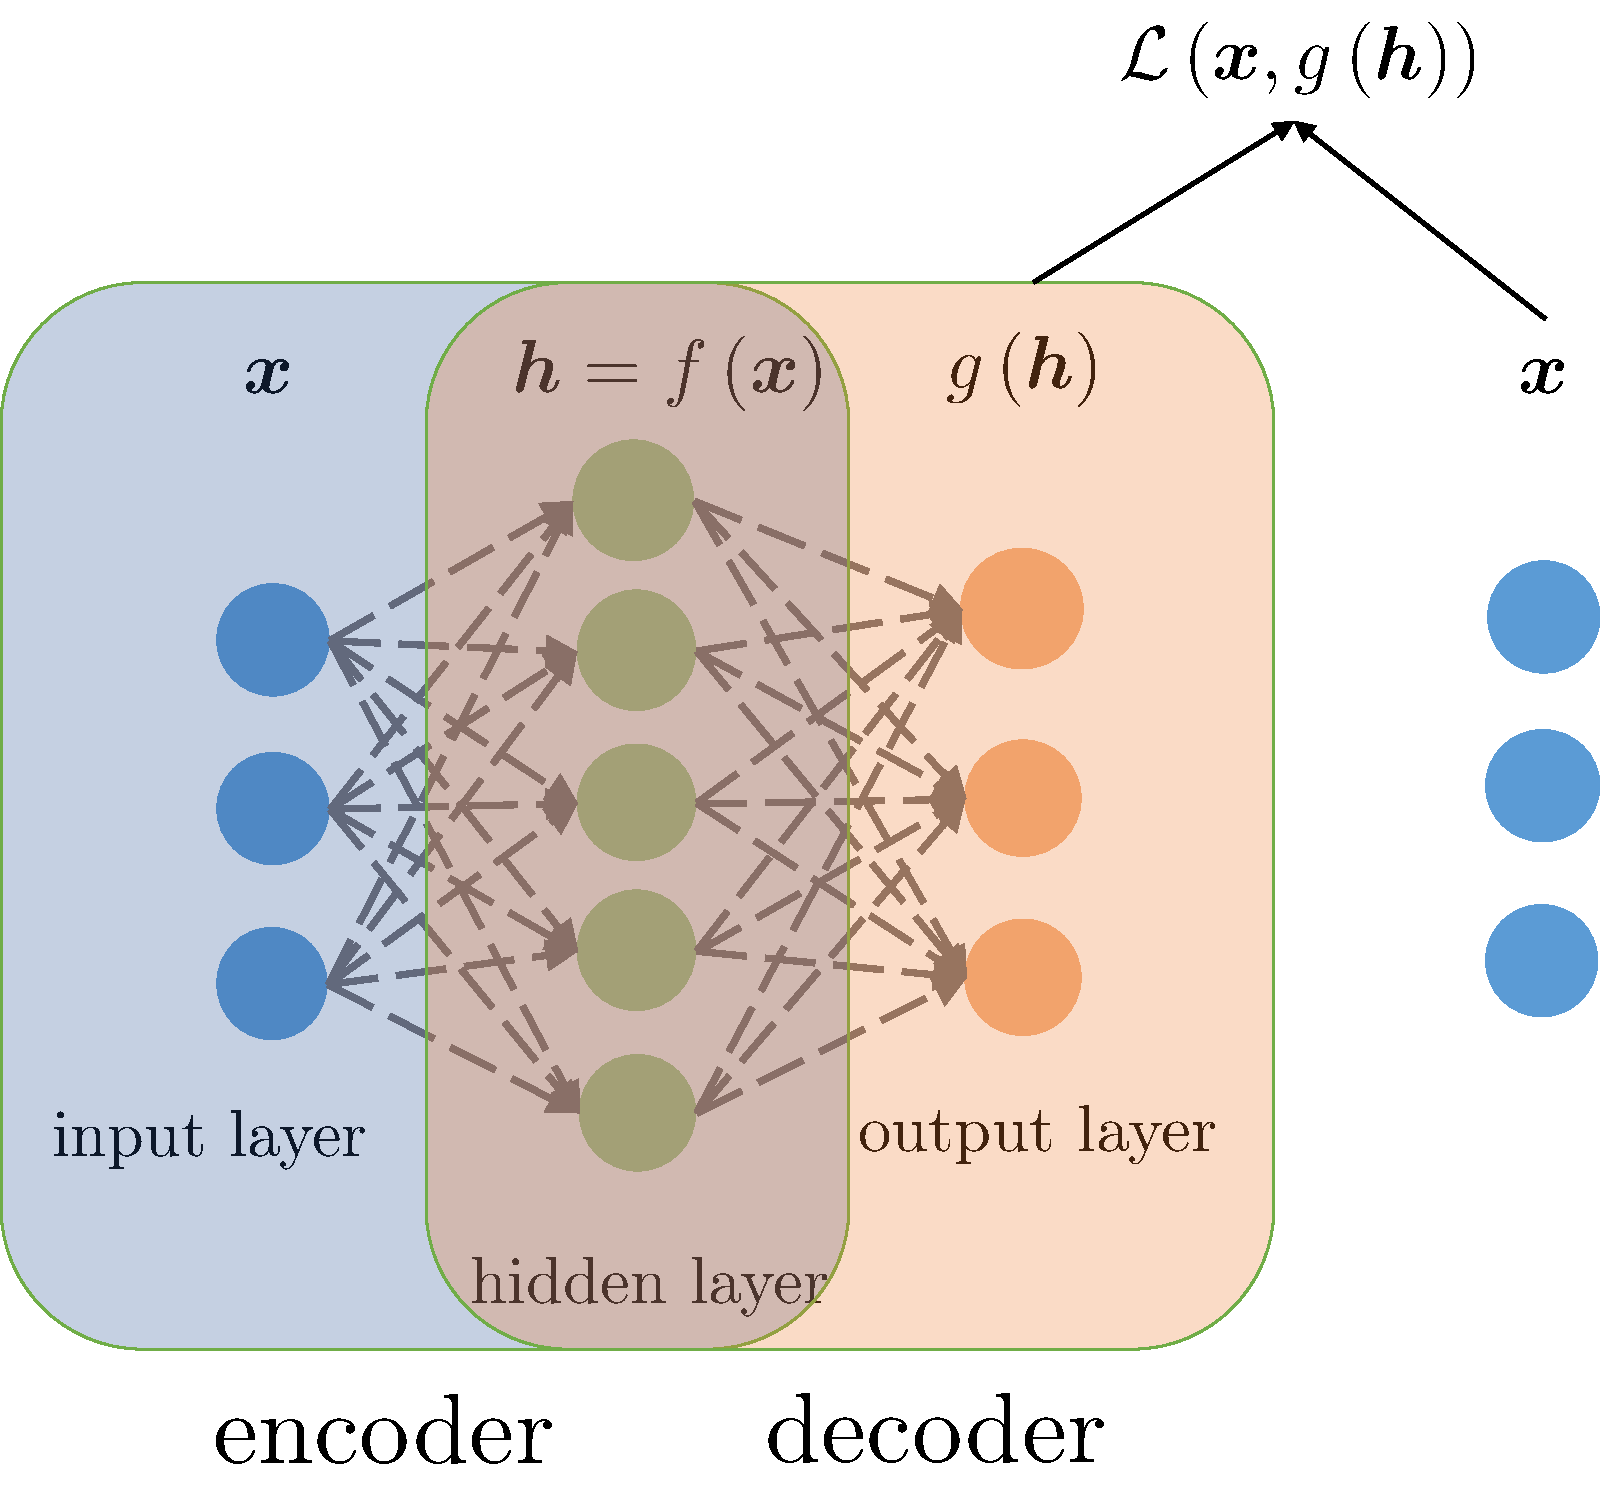
\includegraphics[scale=0.2]{AE}
        \caption{First an input $\bm{x}$ goes through the decoder $\ff(\cdot)$, and we obtain its hidden representation $\bm{h}= \ff(\bm{x})$. Then, we use the decoder $\bgg(\cdot)$ to get $\bgg(\bm{h})$ as a reconstruction of $\bm{x}$. Finally, the loss is determined from the difference between the original input $\bm{x}$ and its reconstruction $\bgg(\ff(\bm{x}))$.}\label{fig:AE} %\TODO{give more than one layer}
    \end{figure}

\end{frame}

\section{Generative adversarial networks}

\begin{frame}
    \frametitle{GAN}
        
    \begin{figure}
        \centering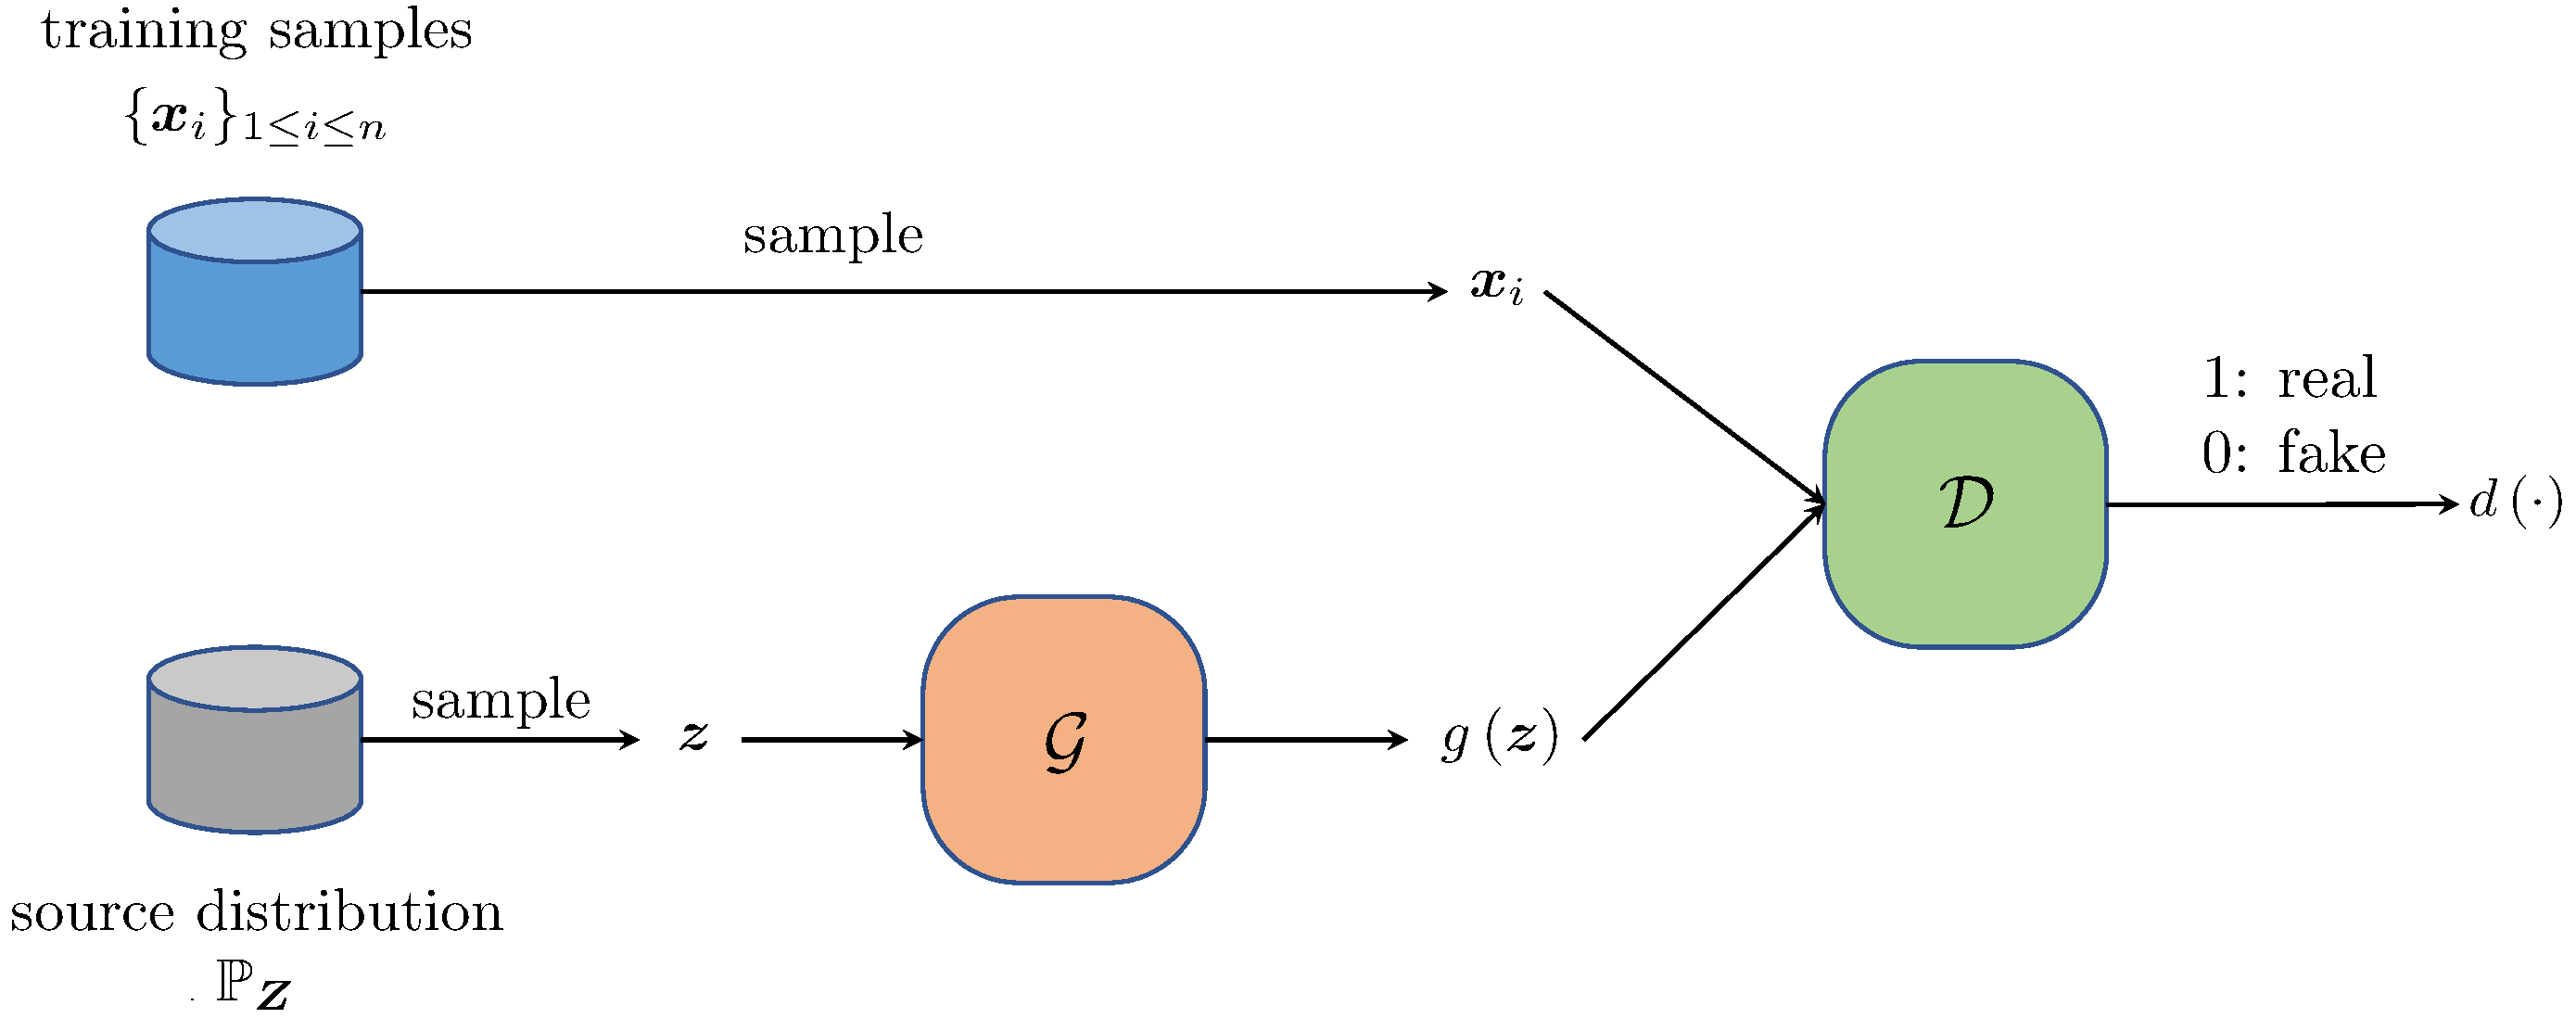
\includegraphics[width=0.9\textwidth]{GAN}
        \caption{GANs consist of two components, a generator $\mathcal{G}$ which generates fake samples and a discriminator $\mathcal{D}$ which differentiate the true ones from the fake ones. \label{fig:GAN}}
    \end{figure}

\end{frame}
\begin{frame}
    \frametitle{GAN}
        
    
    \begin{equation}
        \min_{\btheta_{\mathcal{G}}}\max_{\btheta_{\mathcal{D}}}
        \,\mathbb{E}_{\bm{x}\sim\mathbb{P}_{\bm{X}}}\left[\log
        \left(d\left(\bm{x}\right)\right)\right]
        +\mathbb{E}_{\bm{z}\sim\mathbb{P}_{\bm{Z}}}\left[\log\left(1-d\left(\bg\left(\bm{z}\right)\right)\right)\right].\label{eq:GAN-original}
    \end{equation}
    \pause
    \begin{equation}\label{eq:GAN-new}
        \min_{\mathbb{P}_{\mathcal{G}}}\max_{d(\cdot)}\,\mathbb{E}_{\bm{x}\sim\mathbb{P}_{\bm{X}}}\left[\log\left(d\left(\bm{x}\right)\right)\right]+\mathbb{E}_{\bm{x}\sim\mathbb{P}_{\mathcal{G}}}\left[\log\left(1-d\left(\bm{x}\right)\right)\right].
    \end{equation}
    \pause
    \begin{equation}
        d^{*}\left(\bm{x}\right)=\frac{\mathbb{P}_{\bm{X}}\left(\bm{x}\right)}{\mathbb{P}_{\bm{X}}\left(\bm{x}\right)+\mathbb{P}_{\mathcal{G}}\left(\bm{x}\right)}.
    \end{equation}
    \pause
    \begin{equation}
        \min_{\mathbb{P}_{\mathcal{G}}}\qquad\text{JS}\left(\mathbb{P}_{\bm{X}}\;\|\;\mathbb{P}_{\mathcal{G}}\right)\label{eq:JS-min},
    \end{equation}
    where $\text{JS}(\cdot\|\cdot)$ denotes the Jensen--Shannon divergence
    between two distributions
    \begin{equation}
        \text{JS}\left(\mathbb{P}_{\bm{X}}\|\mathbb{P}_{\mathcal{G}}\right)=\frac{1}{2}\text{KL}\big(\mathbb{P}_{\bm{X}}\;\|\;\tfrac{\mathbb{P}_{\bm{X}}+\mathbb{P}_{\mathcal{G}}}{2}\big)+\frac{1}{2}\text{KL}\big(\mathbb{P}_{\mathcal{G}}\;\|\;\tfrac{\mathbb{P}_{\bm{X}}+\mathbb{P}_{\mathcal{G}}}{2}\big).
    \end{equation}
    it minimizes
    the Wasserstein distance between $\mathbb{P}_{\bm{X}}$ and $\mathbb{P}_{\mathcal{G}}$:
    \begin{equation}
        \min_{\btheta_{\mathcal{G}}}\quad \text{WS}\left(\mathbb{P}_{\bm{X}}\|\mathbb{P}_{\mathcal{G}}\right)\;\;=\;\;\min_{\btheta_{\mathcal{G}}}\sup_{f:f\text{ 1-Lipschitz}}\mathbb{E}_{\bm{x}\sim\mathbb{P}_{\bm{X}}}
        \left[f\left(\bm{x}\right)\right]-\mathbb{E}_{\bm{x}\sim
        \mathbb{P}_{\mathcal{G}}}\left[f\left(\bm{x}\right)\right],\label{eq:WS-GAN}
    \end{equation}

\end{frame}

\begin{frame}[standout]
    Questions
\end{frame}

\end{document}

